%----------------------------------------------------------------------------------------
%	FOCAL PLANE RECONSTRUCTION
%----------------------------------------------------------------------------------------
%\subsection{Methodology}
\label{se:fov}

\begin{figure}[ht]
\begin{center}
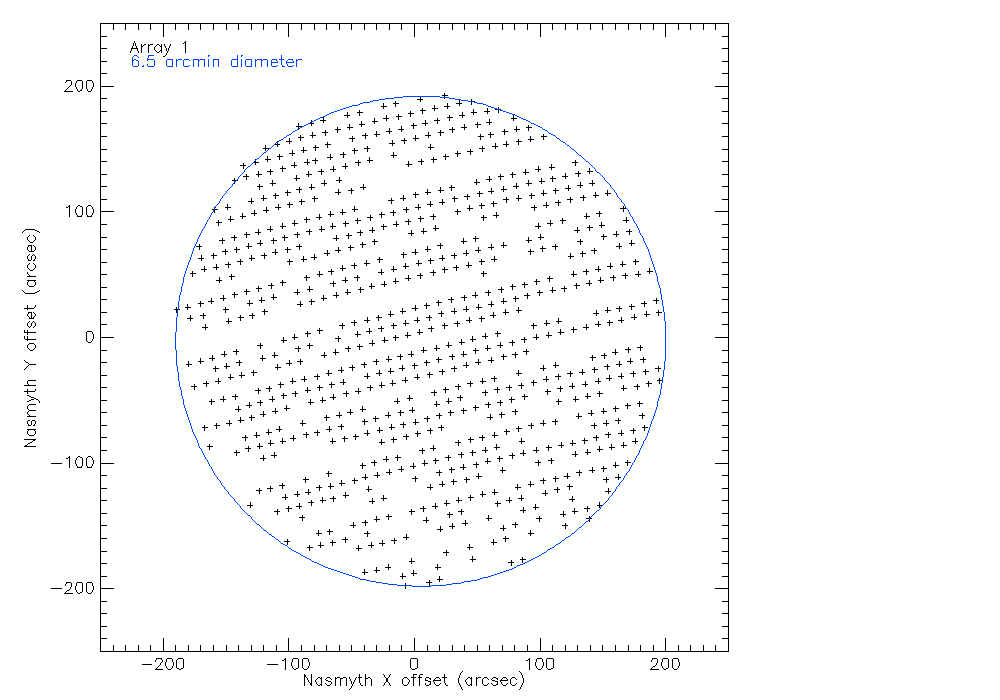
\includegraphics[clip, angle=0, scale = 0.15]{Figures/FOV_A1.png}
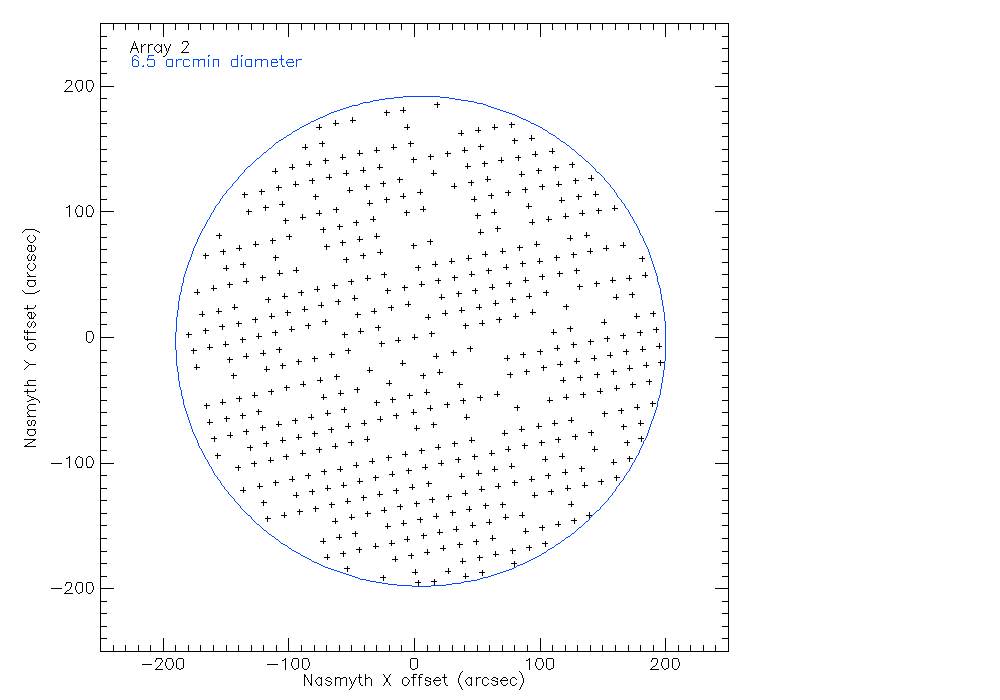
\includegraphics[clip, angle=0, scale = 0.15]{Figures/FOV_A2.png}
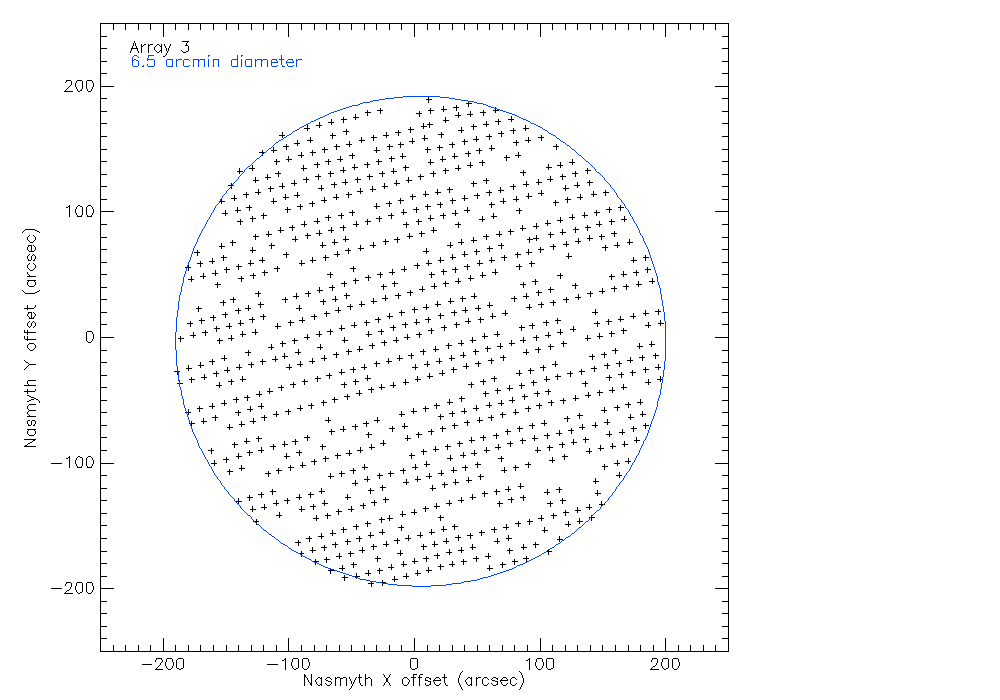
\includegraphics[clip, angle=0, scale = 0.15]{Figures/FOV_A3.png}
\caption{Nasmyth offsets of each array, from beammap 20170226s415 on
  3C84 (N2R9).}
\label{fig:fov_ex}
\end{center}
\end{figure}

% moved to the average FOV section
%\begin{table}
%\begin{tabular}{|l|l|l|}
%\hline
%Array & Number of valid kids & Fraction of all kids\\
%\hline
%A1 & 793 & 0.75\\
%A2 & 481 & 0.83\\
%A3 & 872 & 0.83\\
%\hline
%\end{tabular}
%\end{table}

In order to determine the pointing offsets of each KID w.r.t. the reference sky
coordinates as commanded by the telescope tracking system, we perform a
``beammap'', that is to say we map a bright and compact source, most of the time
a planet, with a elevation step small enough to meet Nyquist sampling at the 1mm
beam scale, namely 4.8~arcsec. We observe this planet with a raster scan in
(az,el) coordinates, either with fixed elevation subscans or fixed azimuth
subscans. The former has the advantage of low air mass variation across a
subscan, the latter offers an orthogonal scan direction to the former: the
combination of both gives a more accurage determination of the far side
lobes. The data reduction proceeds in two steps.

\paragraph{Step 1.} We apply a median filter per
KID timeline whose width is 4~FWHM and we project one map per KID in Nasmyth
coordinates. This median filter removes most of atmospheric and low frequency
electronic noise efficiently, albeit a slight ringing and flux loss on the
source. However, at this stage, we are only interested in the location of the
observed planet. To derive the Nasmyth coordinates from the provided (az,el)
coordinates, we build the following quantities at each time $t$

\begin{eqnarray}
dx_t &=& \cos el_t\, daz_t - \sin el_t\, del_t \nonumber \\
dy_t &=& \sin el_t\, daz_t + \cos el_t\, del_t \nonumber
\end{eqnarray}

where $el_t$ is the elevation of the reference pointing direction and $daz$ and
$del$ are the pointing offsets w.r.t to the source in azimuth and elevation as
provided by the tracking system. Note that $daz$ is already corrected by the
$\cos el_t$ factor to have orthonormal coordinates in the tangent plane of the sky
and be immune to the geodesic convergence at the poles. We then fit a 2D
elliptical gaussian on each kid map. The centroid of this gaussian is a first
estimate of the KID offsets, FWHM's, ellipticity and sensitivity. We apply a
first KID selection by removing outliers to the statistics on these
parameters. We also discard manually KIDs that show a cross-talk counter part on
their map. At the end of this first step, we are ready to move to a second
stage.

\paragraph{Step 2.} With the Nasmyth offsets derived in step 1, we are now able to
mask out the planet in each KID timeline. This mask is centered on the planet
location as seen by each kid, it is circular and has a radius of 60~arcsec. We
now build a template timeline (a.k.a. ``common mode'') in two steps. First, we
take the median of all samples of all KIDs that are outside this mask at a given
time $t$. This gives a first estimate of the common mode. Second, we
cross-calibrate each KID on this common mode when the KID is outside the mask
and we coadd all these KID cross-calibrated timelines when they are outside the
mask to have the final common mode. In this sum, each KID TOI is weighted by the
inverse of its variance outside the mask. Once we have this common mode in hand,
we cross-calibrate each TOI on it outside the mask and we subtract it to the
entire KID TOI. When then resume to the projection of each KID TOI in Nasmyth
coordinates like in step 1, and the 2D elliptical gaussian fit on the each kid
map. The centroid coordinates and the FWHM are now the final parameters that can
be derived on the current scan.

This analysis is repeated on all the beam maps, which provides statistics and
precision on each KID parameter, together with estimates on KID performance stability.

{\bf show a screen capture of Katana.}\\

% LP: j'ajoute une phrase pour referencer la Figure \ref{fig:fov}
We present an example of the FOV reconstruction in Fig.~\ref{fig:fov_ex}.

\begin{equation}
FOV diameter = \sqrt{4 N_{tot. kids} * gridstep^2/\pi}
\end{equation}

{\bf give the values of gridstep (pitch) both in mm and arcsec on the sky}\\

The same definition applies to ``Effective FOV'' to avoid extra multiplication
by the fraction of valid pixels

\begin{equation}
F\lambda = gridstep\times D(30m)/\lambda
\end{equation}

%\subsection{Average Focal Plane Reconstruction}
\label{avg_kidpar}

\begin{figure}
\begin{center}
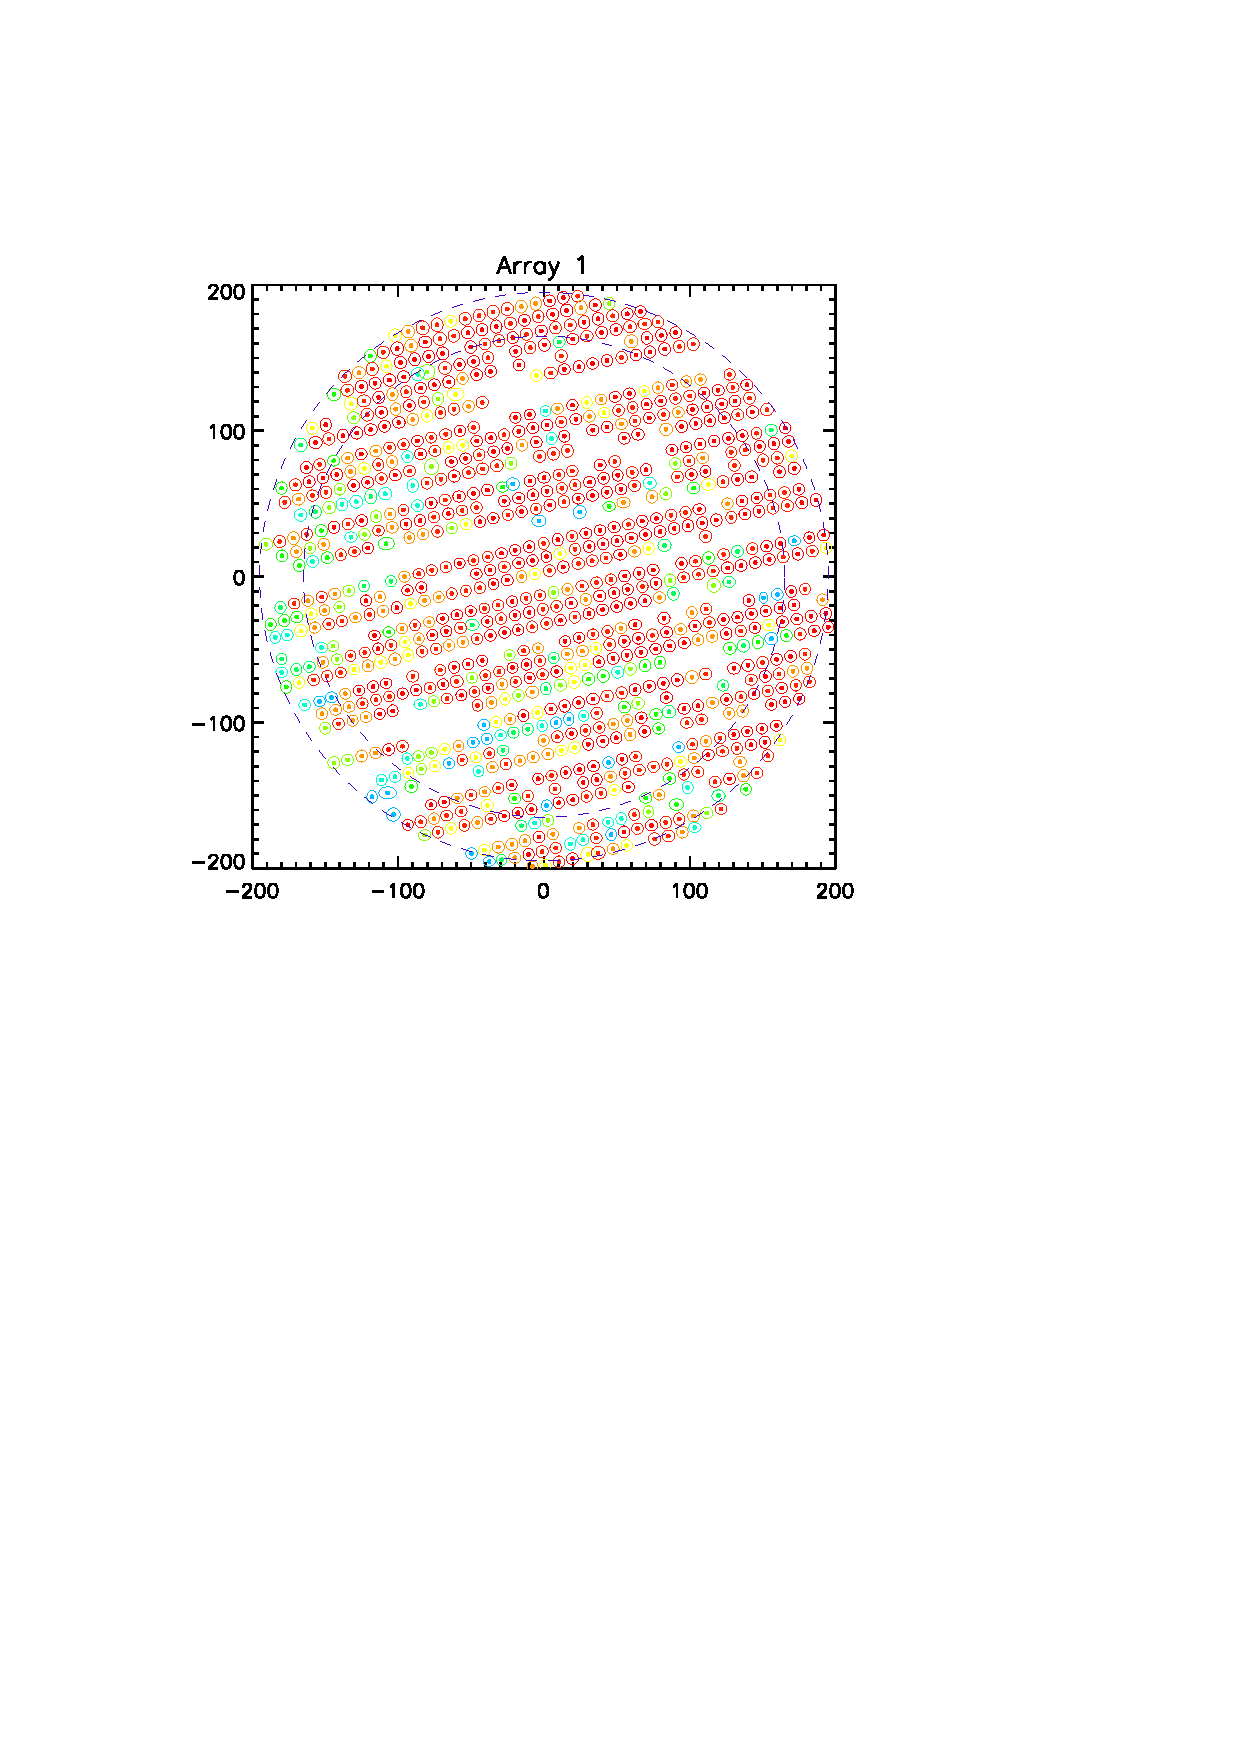
\includegraphics[trim=2cm 14cm 5cm 4cm, clip=true,width=0.6\linewidth]{Figures/A1_fwhm_color_count.pdf}
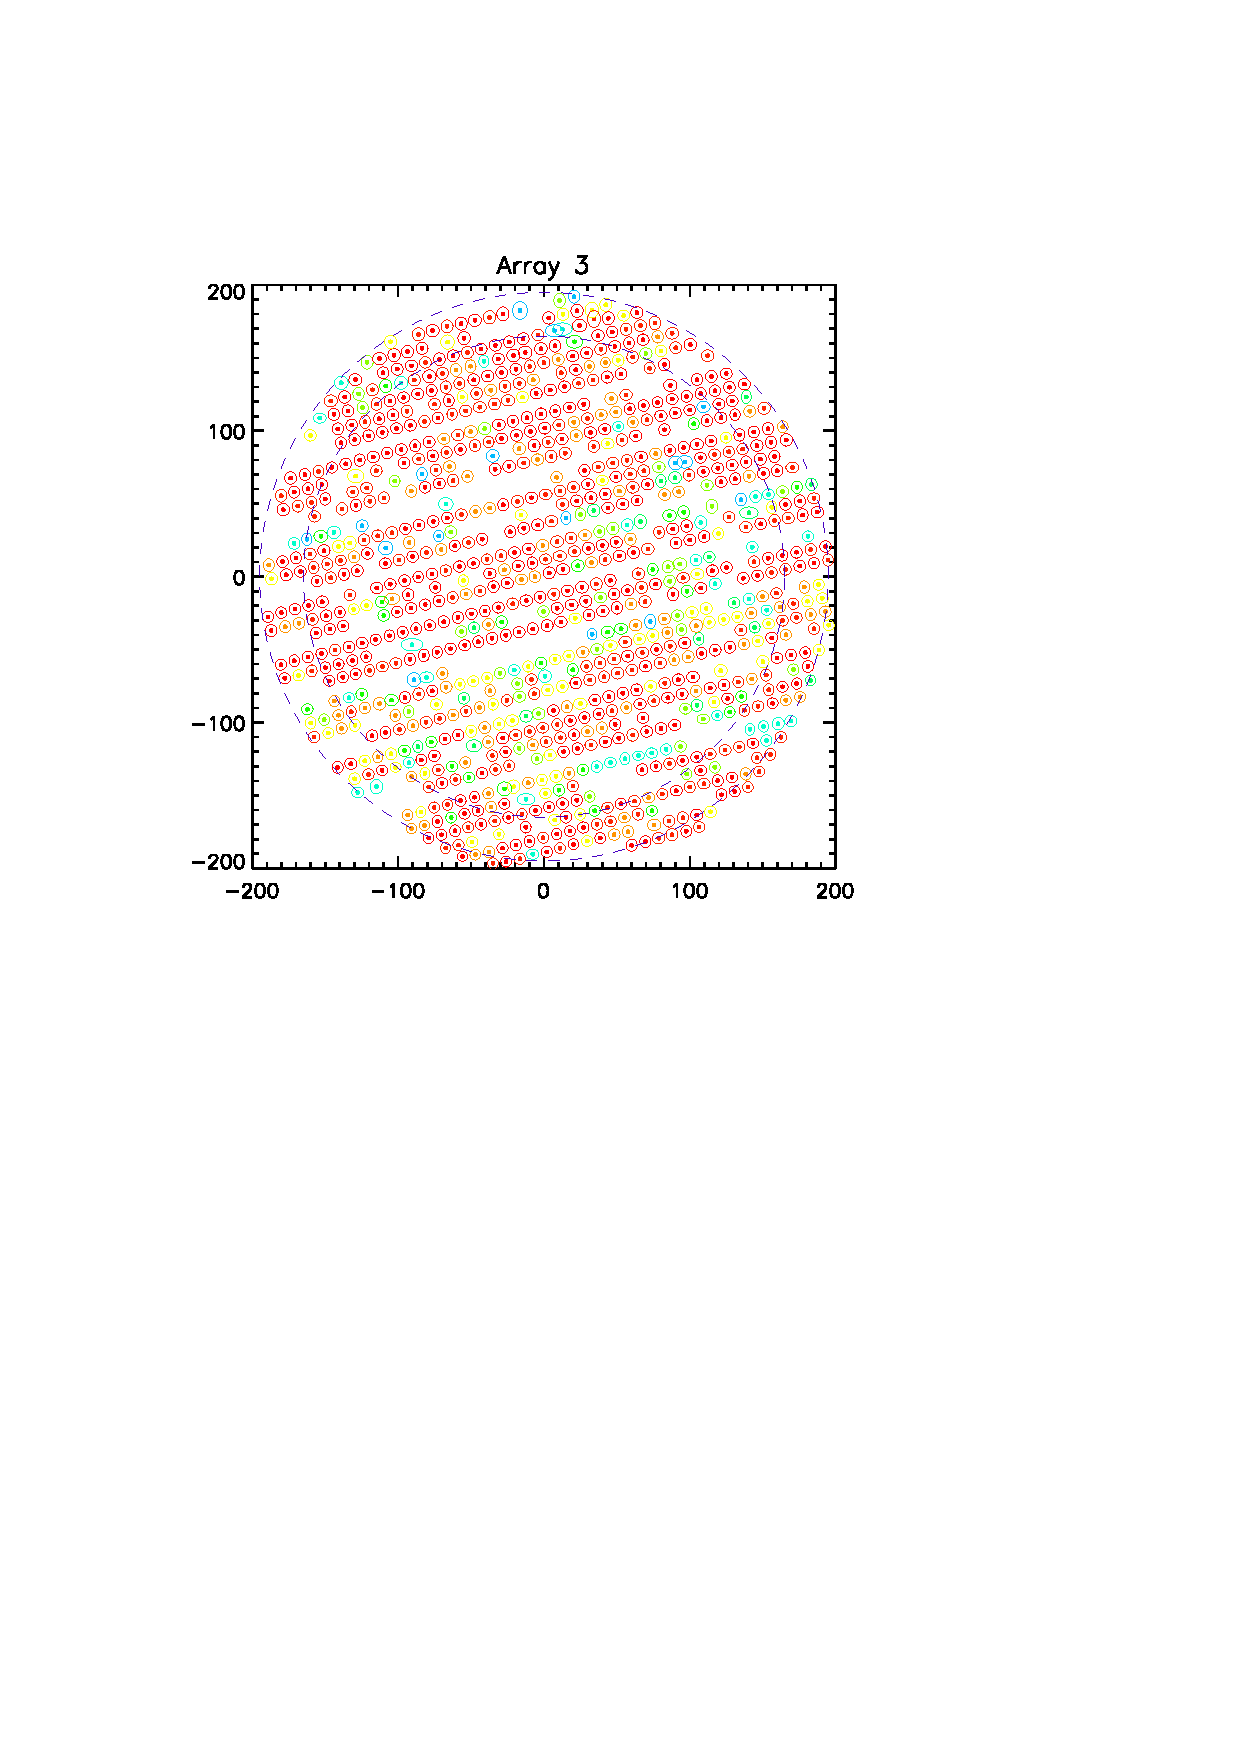
\includegraphics[trim=2cm 14cm 5cm 4cm, clip=true,width=0.6\linewidth]{Figures/A3_fwhm_color_count.pdf}
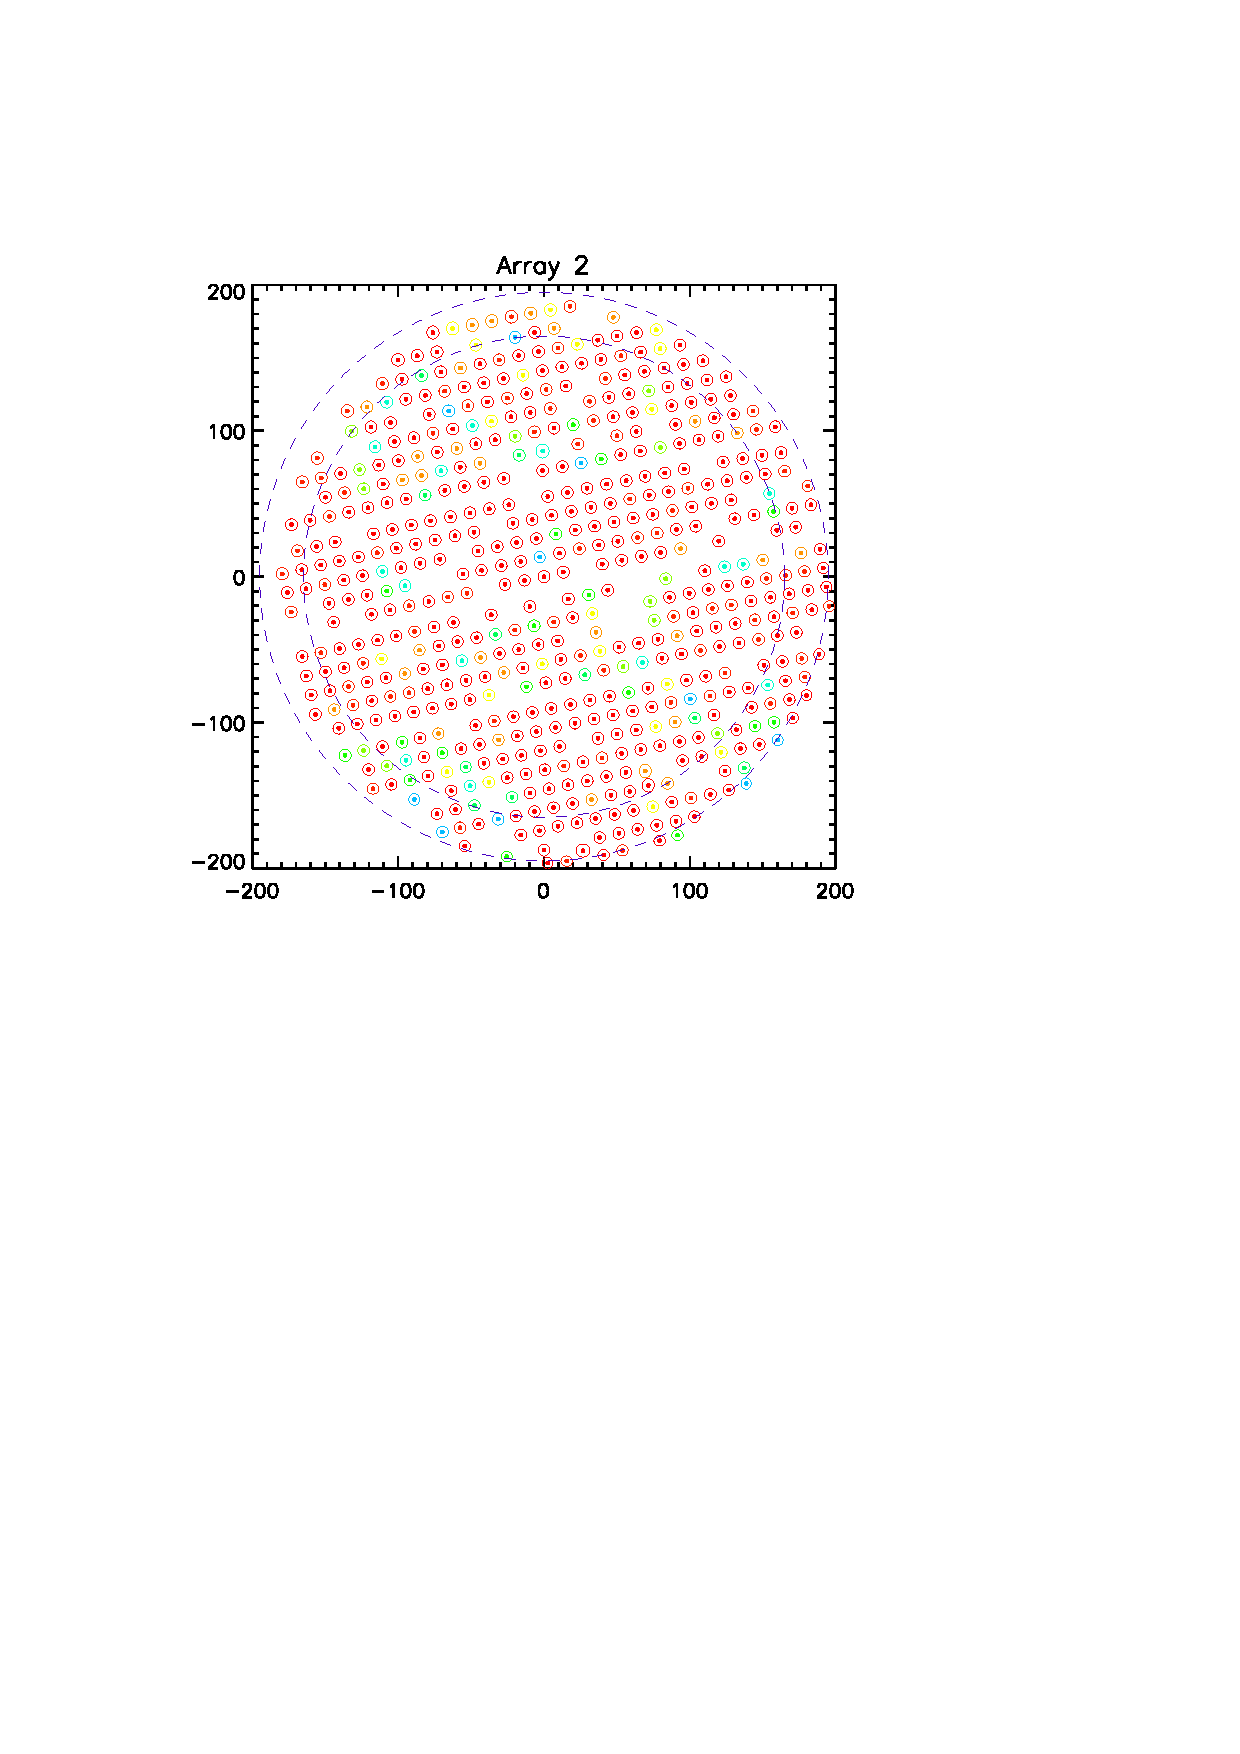
\includegraphics[trim=2cm 14cm 5cm 4cm, clip=true,width=0.6\linewidth]{Figures/A2_fwhm_color_count.pdf}
\caption{Average detectors positions for arrays A1, A3, and A2 (from
  green to red as a function of the number of times that a given pixel
  has been considered as valid). The three plots show the detectors
  that have seen the sky and passed the quality criteria for at least
  two beam maps during Run10, 9 and 8: 952, 961, and 553
  %925, 944, and 543
  for A1, A3 and A2, respectively. The inner and outer dash-line circles correspond to a FOV of 5.5$\prime$ and 6.5$\prime$, respectively. Units are arcseconds. The color (from green to red)  shows the number of times that a given pixel has been considered as valid.}
\label{fig:avg_fov_color}
\end{center}
\end{figure}

In order to identify the most stable pixels, we compare the KIDs parameter obtained with several beam maps. 
In the following we will show results as obtained using seven beam maps from Run10, two from Run9 and one from Run8.
For each pixel we compute the average position on the focal plane and the average FWHM, counting the times that it has been considered as valid.

In Fig. \ref{fig:avg_fov_color} we show the average focal plane
reconstruction, from green to red depending on the number of times
that the pixel has been considered as valid. For A1, A3 and A2,
respectively, we have 952, 961, and 553 pixels that have been
considered as valid at least twice (840, 508, 868 valid at least five
times).
% LP: add a sentence to reference Table ``\ref{tab:number_of_kids}"
Using this criterion, we deduce the fraction of valid
detectors over the designed ones, as given in Table~\ref{tab:number_of_kids}. 
As a second step, we also flag pixels that move across the focal plane from a beam map to another (Fig. \ref{fig:jumping_kids} , jumping KIDs) and those who share the same position (twin KIDs). To identify the former we look at the difference of the mean and median position of each KID (the red crosses and black squares in Fig. \ref{fig:mean_vs_median}). For the latter a criteria on the position is applied in order to find the pixels that are closer than the grid step.

\begin{figure}
\begin{center}
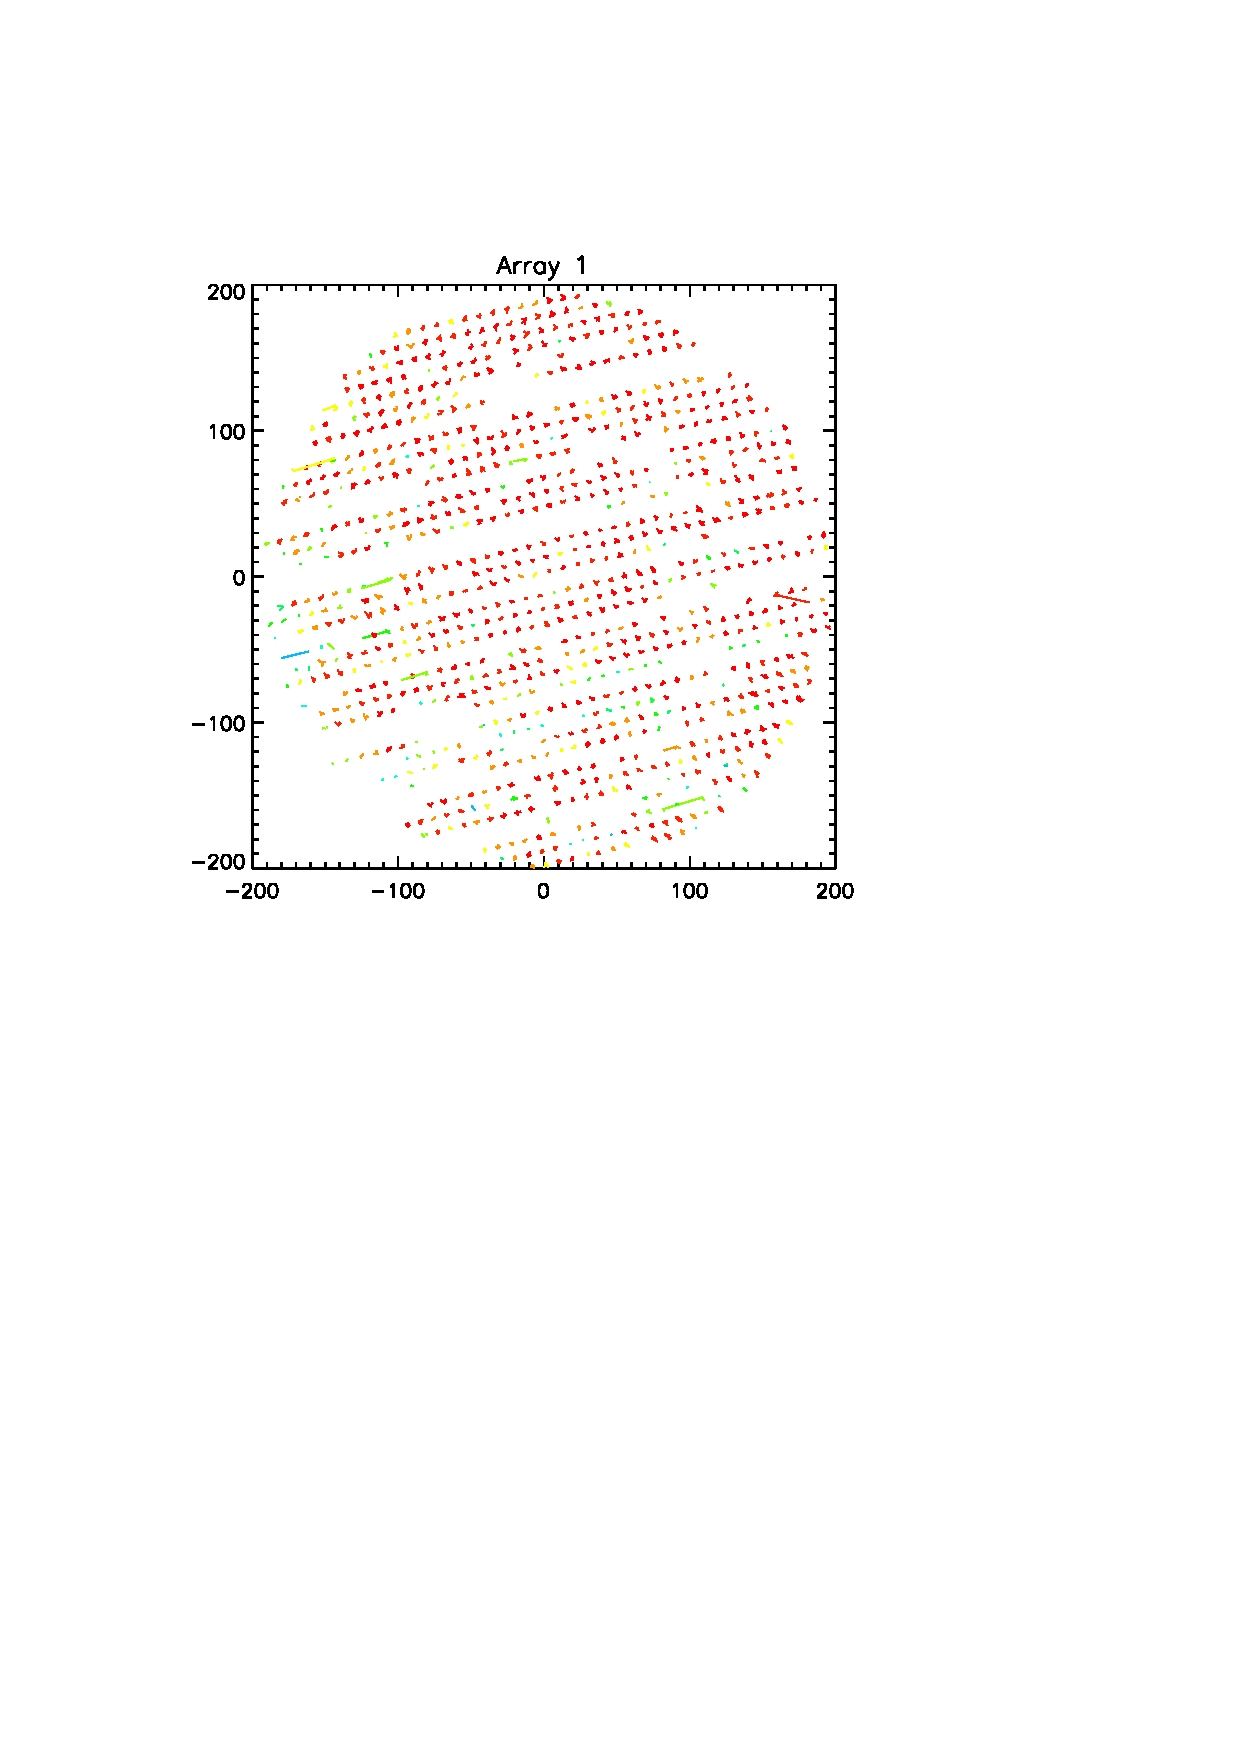
\includegraphics[trim=2cm 14cm 5cm 4cm, clip=true,width=0.6\linewidth]{Figures/A1_positions.pdf}
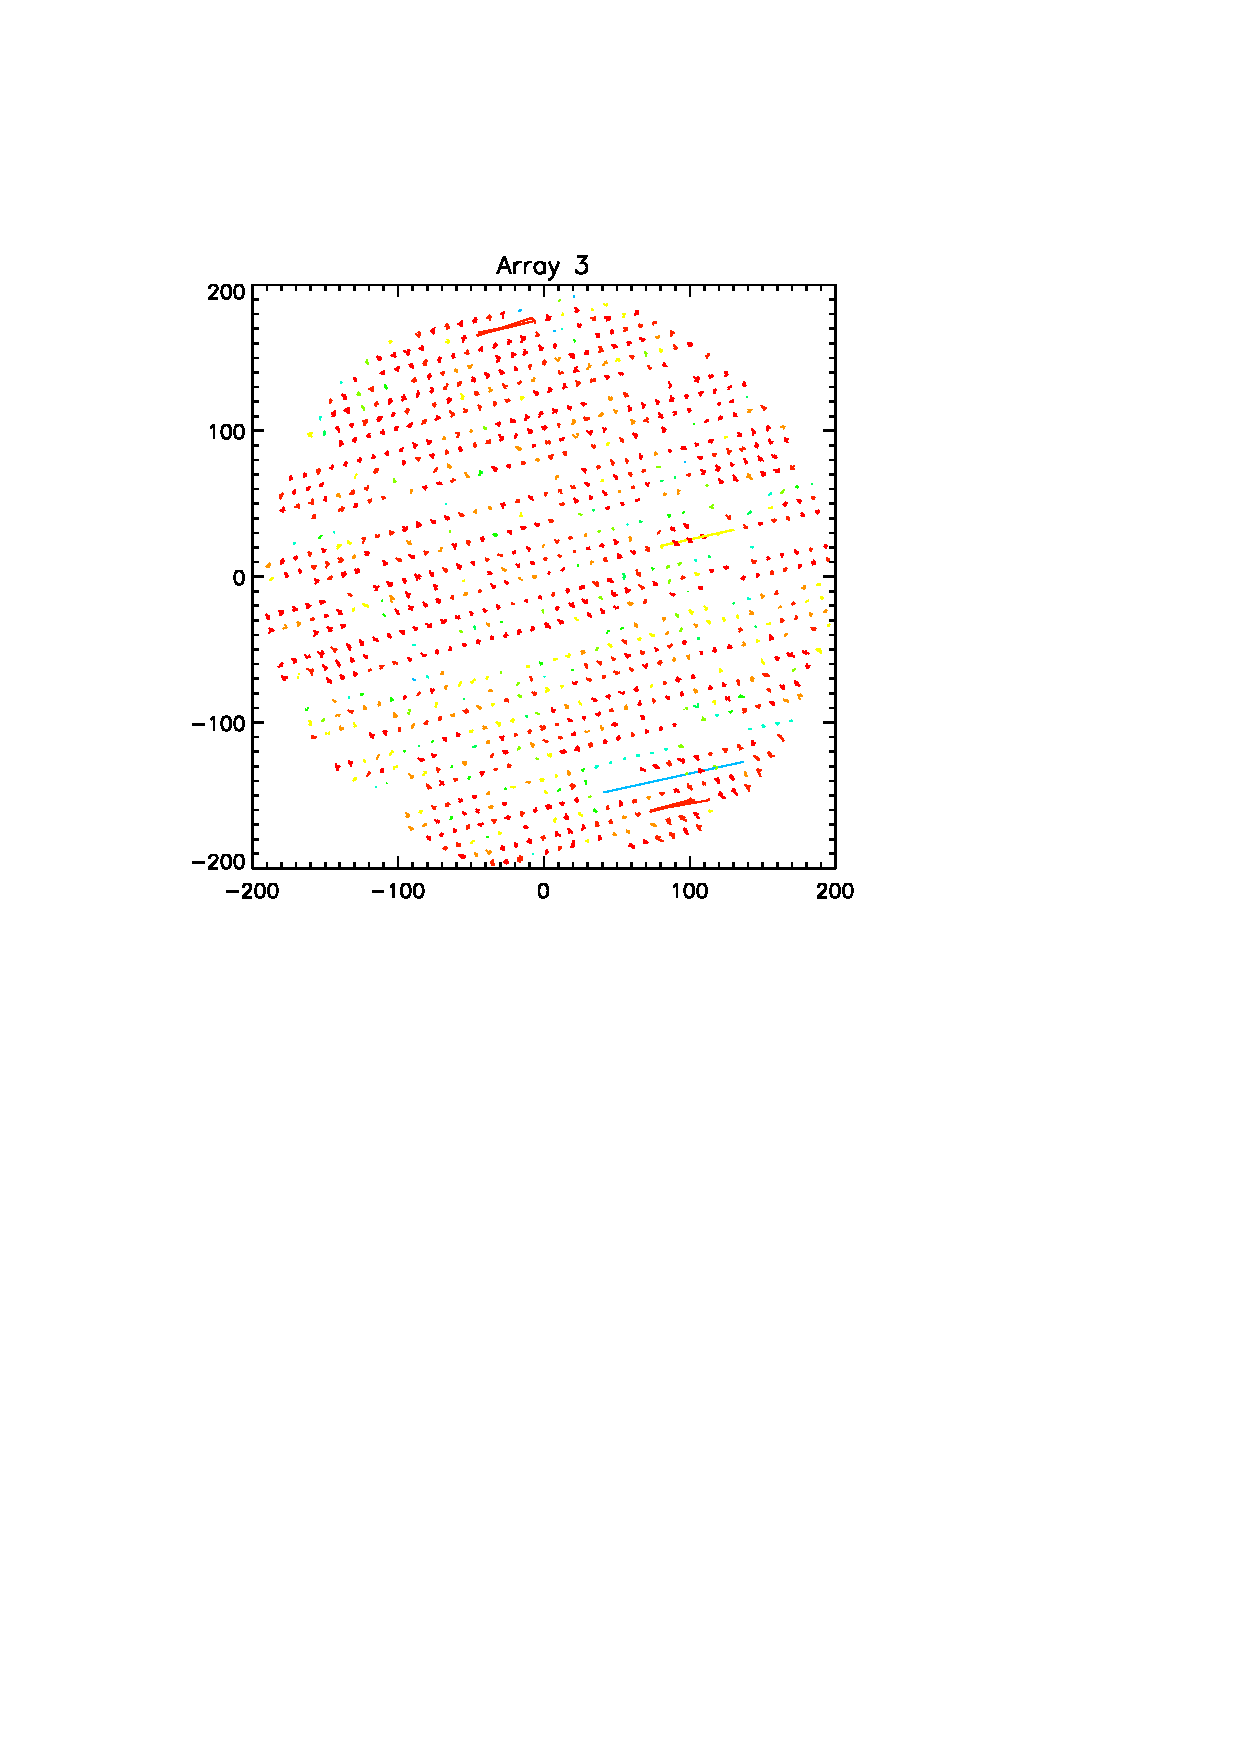
\includegraphics[trim=2cm 14cm 5cm 4cm, clip=true,width=0.6\linewidth]{Figures/A3_positions.pdf}
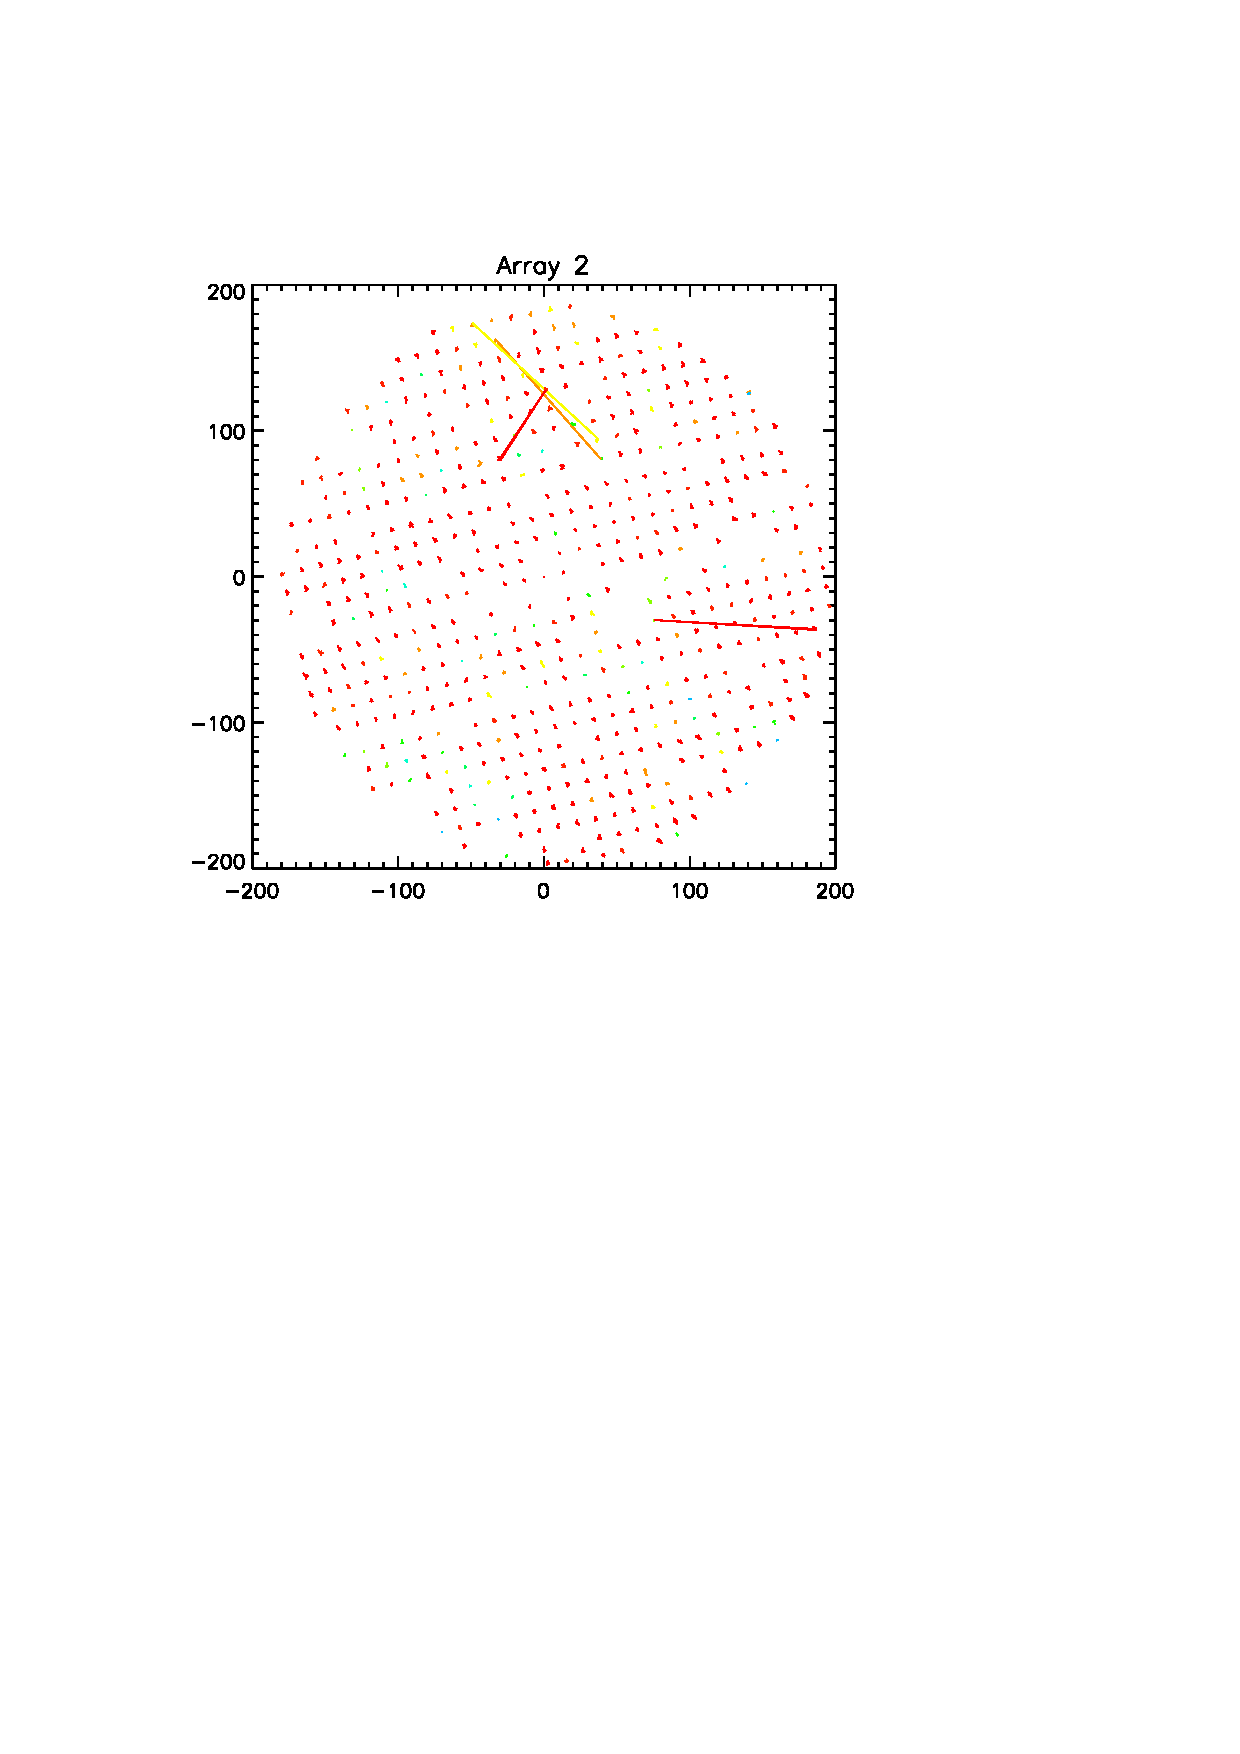
\includegraphics[trim=2cm 14cm 5cm 4cm, clip=true,width=0.6\linewidth]{Figures/A2_positions.pdf}
\caption{For the 952, 961, and 553 pixels that have passed the quality criteria at least twice for A1, A3 and A2, we show the positions of each pixel, as obtained from each beam map. We can see that some of them are not found at the same position for all the beam maps. Units are arcseconds.}
\label{fig:jumping_kids}
\end{center}
\end{figure}

\begin{figure}
\begin{center}
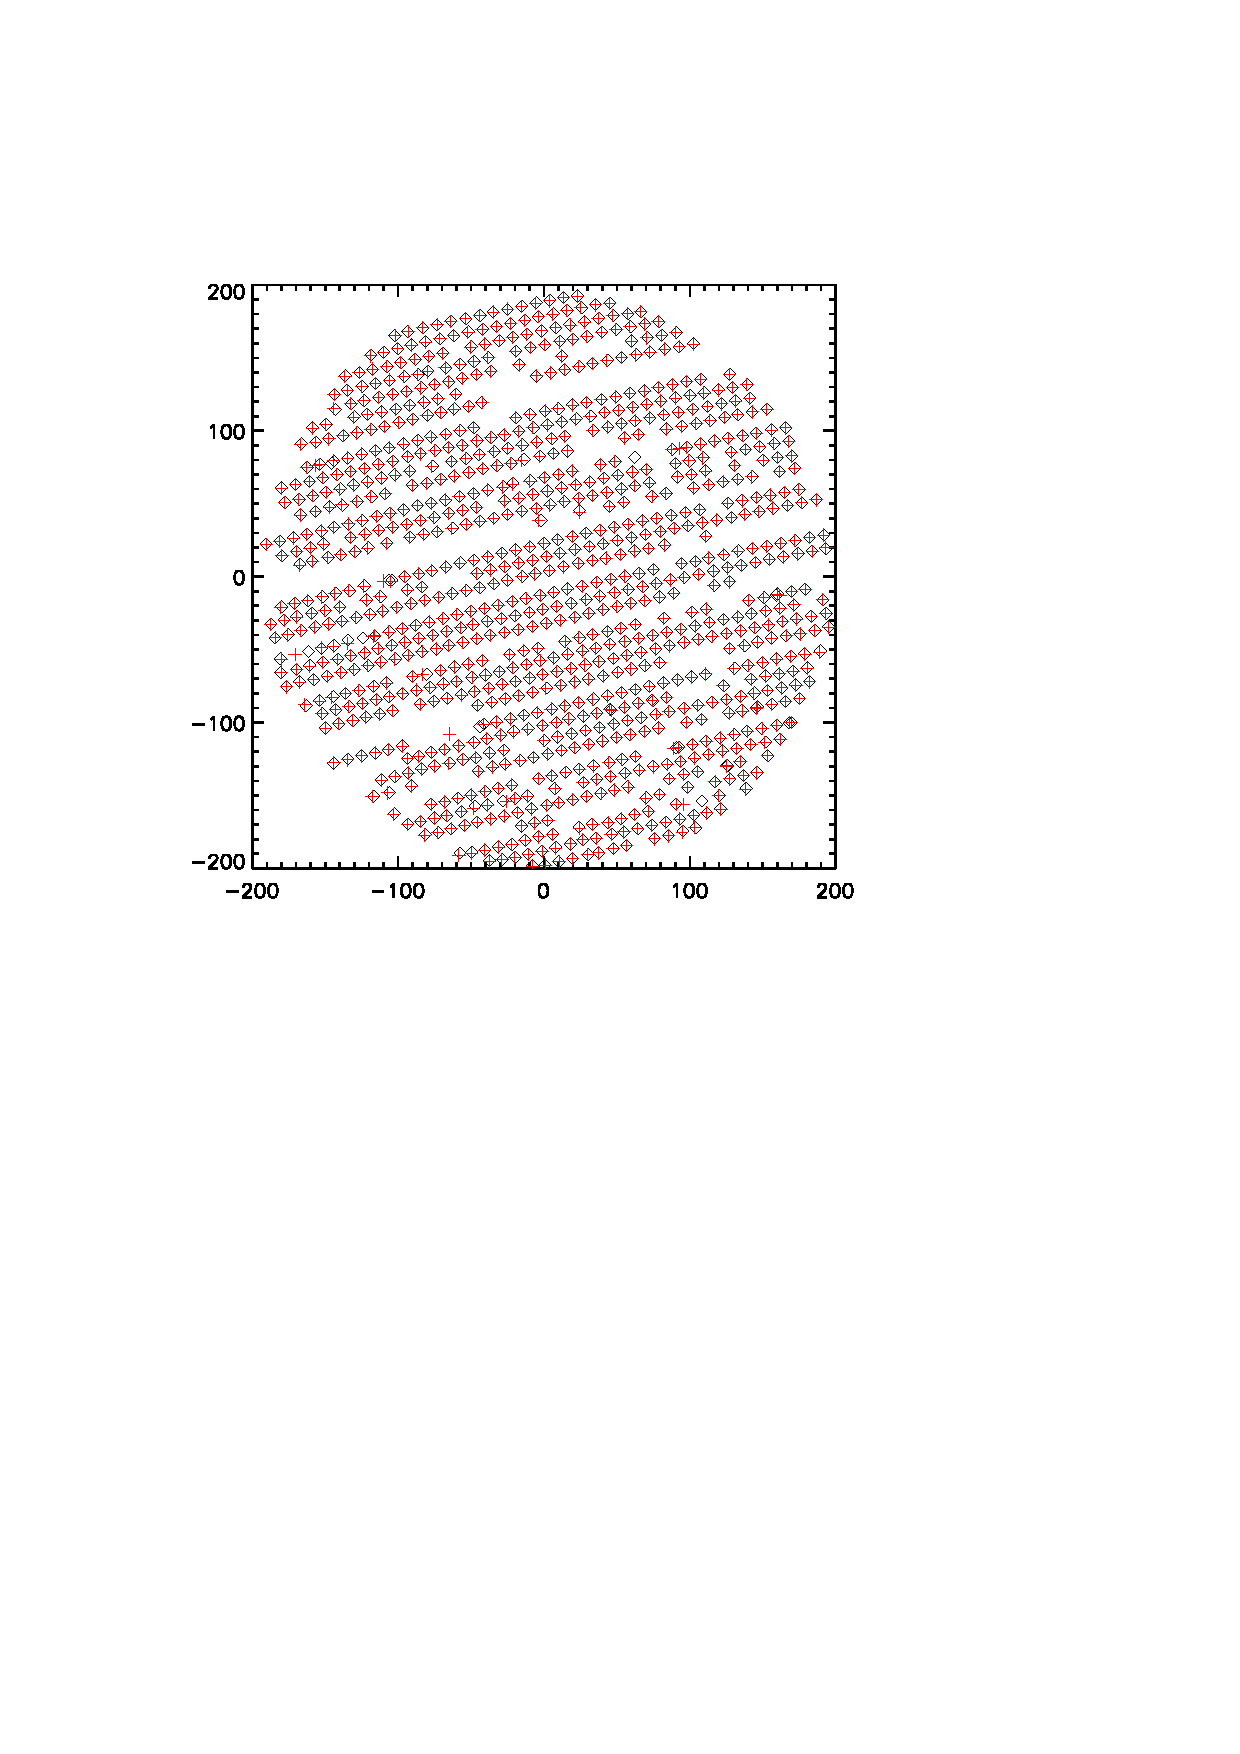
\includegraphics[trim=2cm 14cm 5cm 4cm, clip=true,width=0.6\linewidth]{Figures/A1_test_positions.pdf}
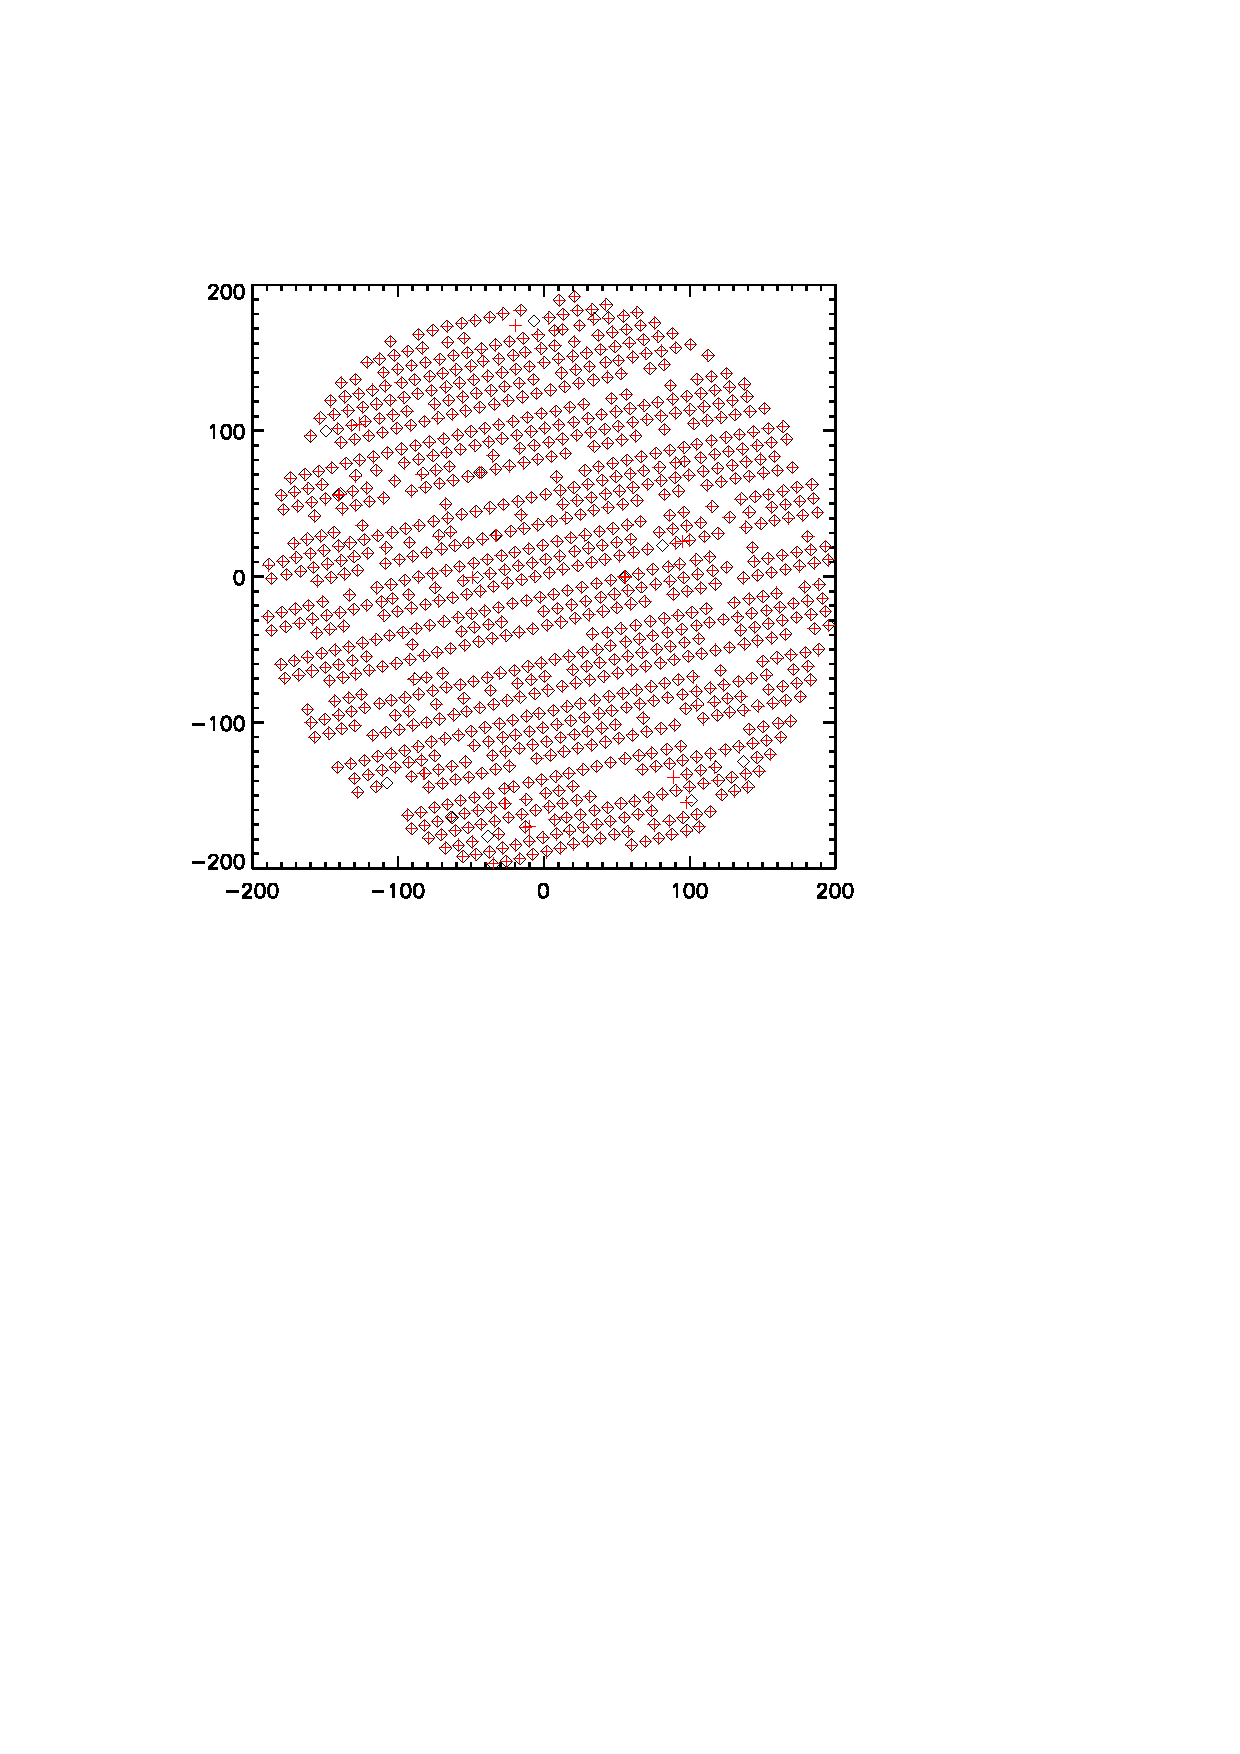
\includegraphics[trim=2cm 14cm 5cm 4cm, clip=true,width=0.6\linewidth]{Figures/A3_test_positions.pdf}
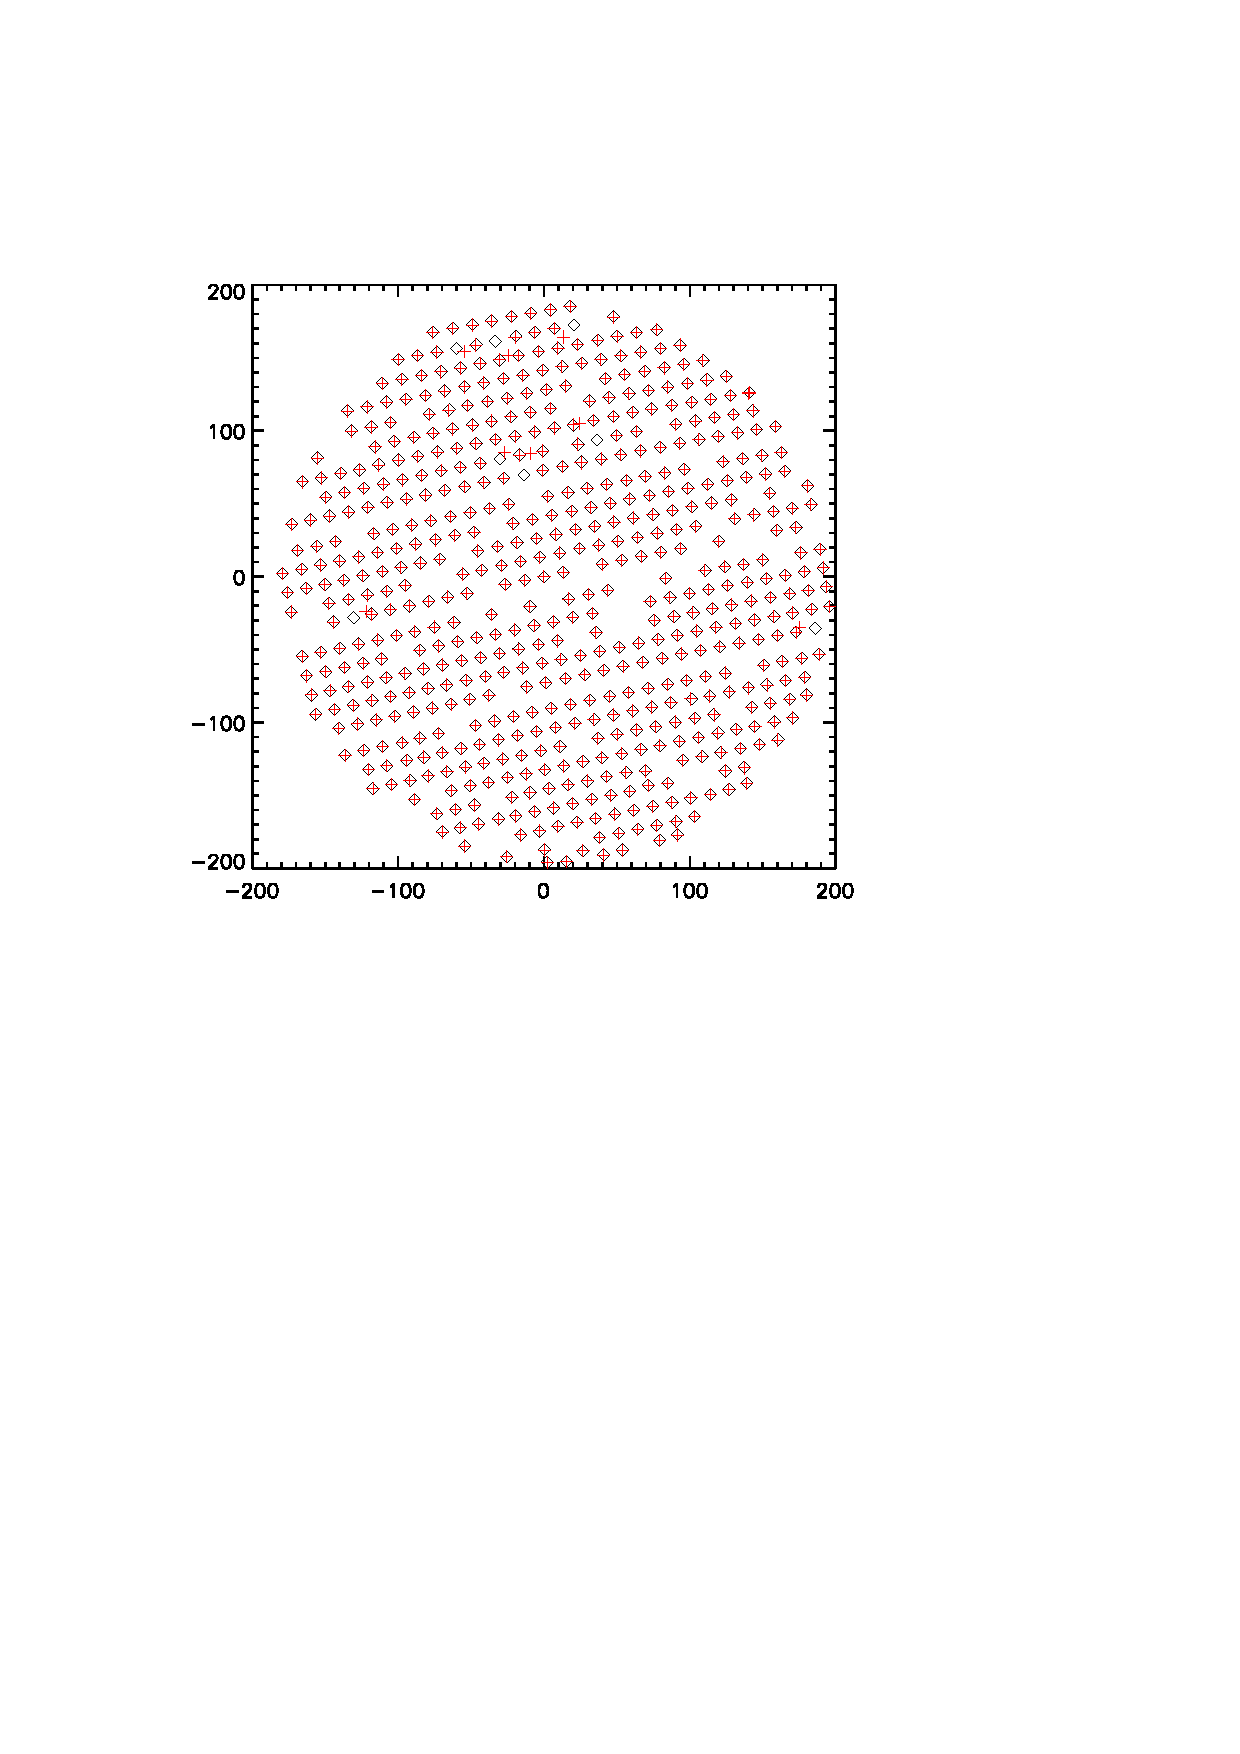
\includegraphics[trim=2cm 14cm 5cm 4cm, clip=true,width=0.6\linewidth]{Figures/A2_test_positions.pdf}
\caption{For the 952, 961, and 553 pixels that
  have passed the quality criteria at least twice for A1, A3 and A2,
  we show the mean (red crosses) and the median (black squares)
  positions of each pixel, as obtained from each beam map.
  Units are arcseconds. }
\label{fig:mean_vs_median}
\end{center}
\end{figure}


% LP: copy from fov.tex + modif according to Samuel's comment
\begin{table}
  \label{tab:number_of_kids}
  \begin{tabular}{|r|r|r|r|}
    \hline
    Array & Number of designed detectors &  Number of valid detectors & Fraction of all detectors\\
    \hline
    A1 & 1140 & 952 &  0.84\\
    A3 & 1140 & 961 &  0.84\\
    A2 & 616  & 553 &  0.90\\
    \hline
  \end{tabular}
\end{table}

%\subsection{FOV grid distortion}
\label{se:grid_distortion}

{\bf LP edit using Samuel's comments, [TBC]}

We studied the matching of the KIDs position on the sky to the
\emph{design} position, as decribed in Xavier's wiki post\footnote{see
  {\tt http$://$www.iram.fr$/$wiki$/$nika2$/$index.php$/$}
  
  {\tt April$\_$19,$\_$2017,$\_$FXD,$\_$KID$\_$position$\_$mapping$\_$and$\_$Field$\_$distortion$\_$for$\_$Run9}
}

This has been compared to expectations obtained using ZEMAX
simulation. The grid diagram generated using ZEMAX provides us with
the maximum dispersion in the field defined by

\begin{equation}
P = \frac{\sqrt{(x_p - x_r)^2 + (y_p - y_r)^2}}{\sqrt{x_p^2 + y_p^2}},
\end{equation}

where $(x_p, y_p)$ and $(x_r, y_r)$ are respectivelly the predicted
and real coordinates on the image surface relative to the reference
field position image location (see page 170 of the ZEMAX manual, 2007).
The predicted coordinates for the whole field are obtained using a
linear interpolation of a small area in the field central part,
whereas the real coordinates are calculated by ray tracing through the
optical system.

\begin{figure}[ht] 
\begin{center}
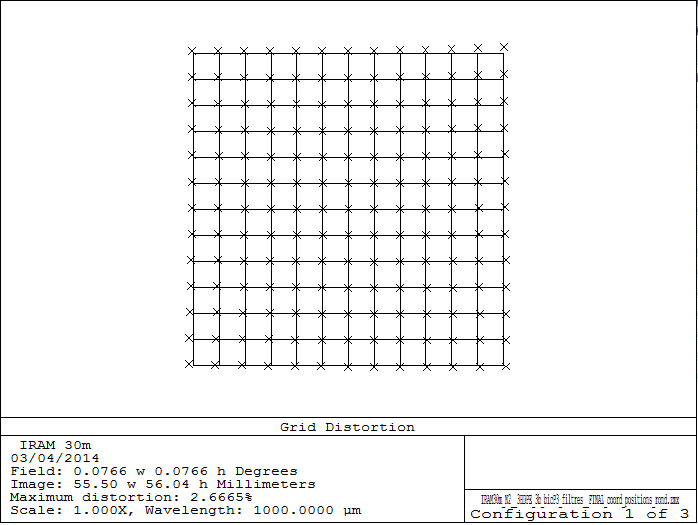
\includegraphics[width=0.9\textwidth]{Figures/NIKA2_Final_grid.png}
\caption{NIKA2 grid diagram simulated using ZEMAX. Crosses indicate
  the real coordinates on the Nasmyth image plan. {\bf question a
    Samuel: pourquoi les dimensions indiquees sont environs 4.5 arcmin
  de cote (et pas 6.5)?}}
 \label{fig:fov_grid_distortion_zemax}
\end{center}
\end{figure}

Figure \ref{fig:fov_grid_distortion_zemax} show the ZEMAX grid diagram for
NIKA2 simulated optic system. The maximum grid distortion is expected
to be of $2.7\%$ in NIKA2 $6.5'$ FOV. The distortion is the most
noticeable in the upper right corner of the Nasmyth plan, which is
also the area of the largest defocus w.r.t. to the center. 



%   Geometry
%----------------------------------------------------------------------------------------
\section{Focal Plane Geometry}% {\color{YellowGreen} Nico}}
\label{se:fov_geometry}

%% \todo{Refer to Sect.~\ref{se:fov_first_geometry} and then present here the
%% results of the combined analysis of all the \bms.}\\
%% 
%% % LP: j'ajoute une phrase pour referencer la Figure \ref{fig:fov}
%% We present an example of the FOV reconstruction in Fig.~\ref{fig:fov_ex}.
%% 
%% The FOV diameter is defined as 
%% \begin{equation}
%% FOV diameter = \sqrt{4 N_{tot. kids} \times gridstep^2/\pi}
%% \end{equation}
%% 
%% {\bf give the values of gridstep (pitch) both in mm and arcsec on the sky}\\
%% 
%% The same definition applies to ``Effective FOV'' to avoid extra multiplication
%% by the fraction of valid pixels
%% 
%% \begin{equation}
%% F\lambda = gridstep\times D(30m)/\lambda
%% \end{equation}

%\subsection{Focal plane geometry reconstruction}
%\label{se:fov_first_geometry}

In order to be able to produce a map, one needs to associate a pointing
direction to any data sample of the system. The telescope provides us with
various pointing information for a reference position in the focal plane. We
then need to know the relative pointing offsets of each detector. We use
\bms\ for this purpose (see Sect.~\ref{se:beammaps}). The determination of the
KID offsets in the focal plane proceeds in two steps.

\paragraph{Step 1.} We apply a median filter per
KID timeline whose width is equivalent to 4~FWHM and we project one
map per KID in Nasmyth coordinates. This median filter removes
efficiently most of the atmospheric and low frequency electronic
noise, albeit with a slight ringing and flux loss on the
source. However, at this stage, we are only interested in the location
of the observed planet. To derive the Nasmyth coordinates from the
provided $(\alpha_t,\delta_t)$ and $(\Delta\alpha_t,\Delta\delta_t)$
coordinates, we build the following quantities at time~$t$ :

\begin{eqnarray}
\Delta x_t &=& \cos\delta_t \Delta\alpha_t - \sin \delta_t\Delta \delta_t \nonumber \\
\Delta y_t &=& \sin\delta_t \Delta\alpha_t + \cos \delta_t\Delta \delta_t \nonumber
\end{eqnarray}

Note that $\Delta\alpha_t$ is already corrected by the $\cos\delta_t$ factor to
have orthonormal coordinates in the tangent plane of the sky and be immune to
the geodesic convergence at the poles. We then fit a 2D elliptical Gaussian on
each kid map. The centroid of this Gaussian is a first estimate of the KID
offsets, FWHM's, ellipticity and sensitivity. We apply a first KID selection by
removing outliers to the statistics on these parameters. We also discard
manually KIDs that show a cross-talk counterpart on their map.

\paragraph{Step 2.} With these offsets, it is already possible to produce maps
from the combination of all detectors. However, in order to go up to
the calibration stage, we must correct for the flux loss induced by
the median filter and ensure that each timeline is treated in the same
way as the final observation will. For this, we apply the pointing
reconstruction presented in Sect.~\ref{se:ptg} and the data reduction
presented in Sect.~\ref{se:toi_proc}. We still do not have absolute
calibration for each KID (no opacity correction yet) but the amplitude
of the fitted centroid on the same planet provides the required
cross-calibration between KIDs. The final absolute calibration will be
presented in Sect.~\ref{se:calibration}.\\

This analysis is repeated on all \bms\ to obtain statistics and
precision on each KID parameter, together with estimates on KID
performance stability, as discussed in the next sections.

%\section{KID selection and average geometry {\color{blue} Nico (Barbara's part)} }
%\label{avg_kidpar}

\begin{figure}[p]
\begin{center}
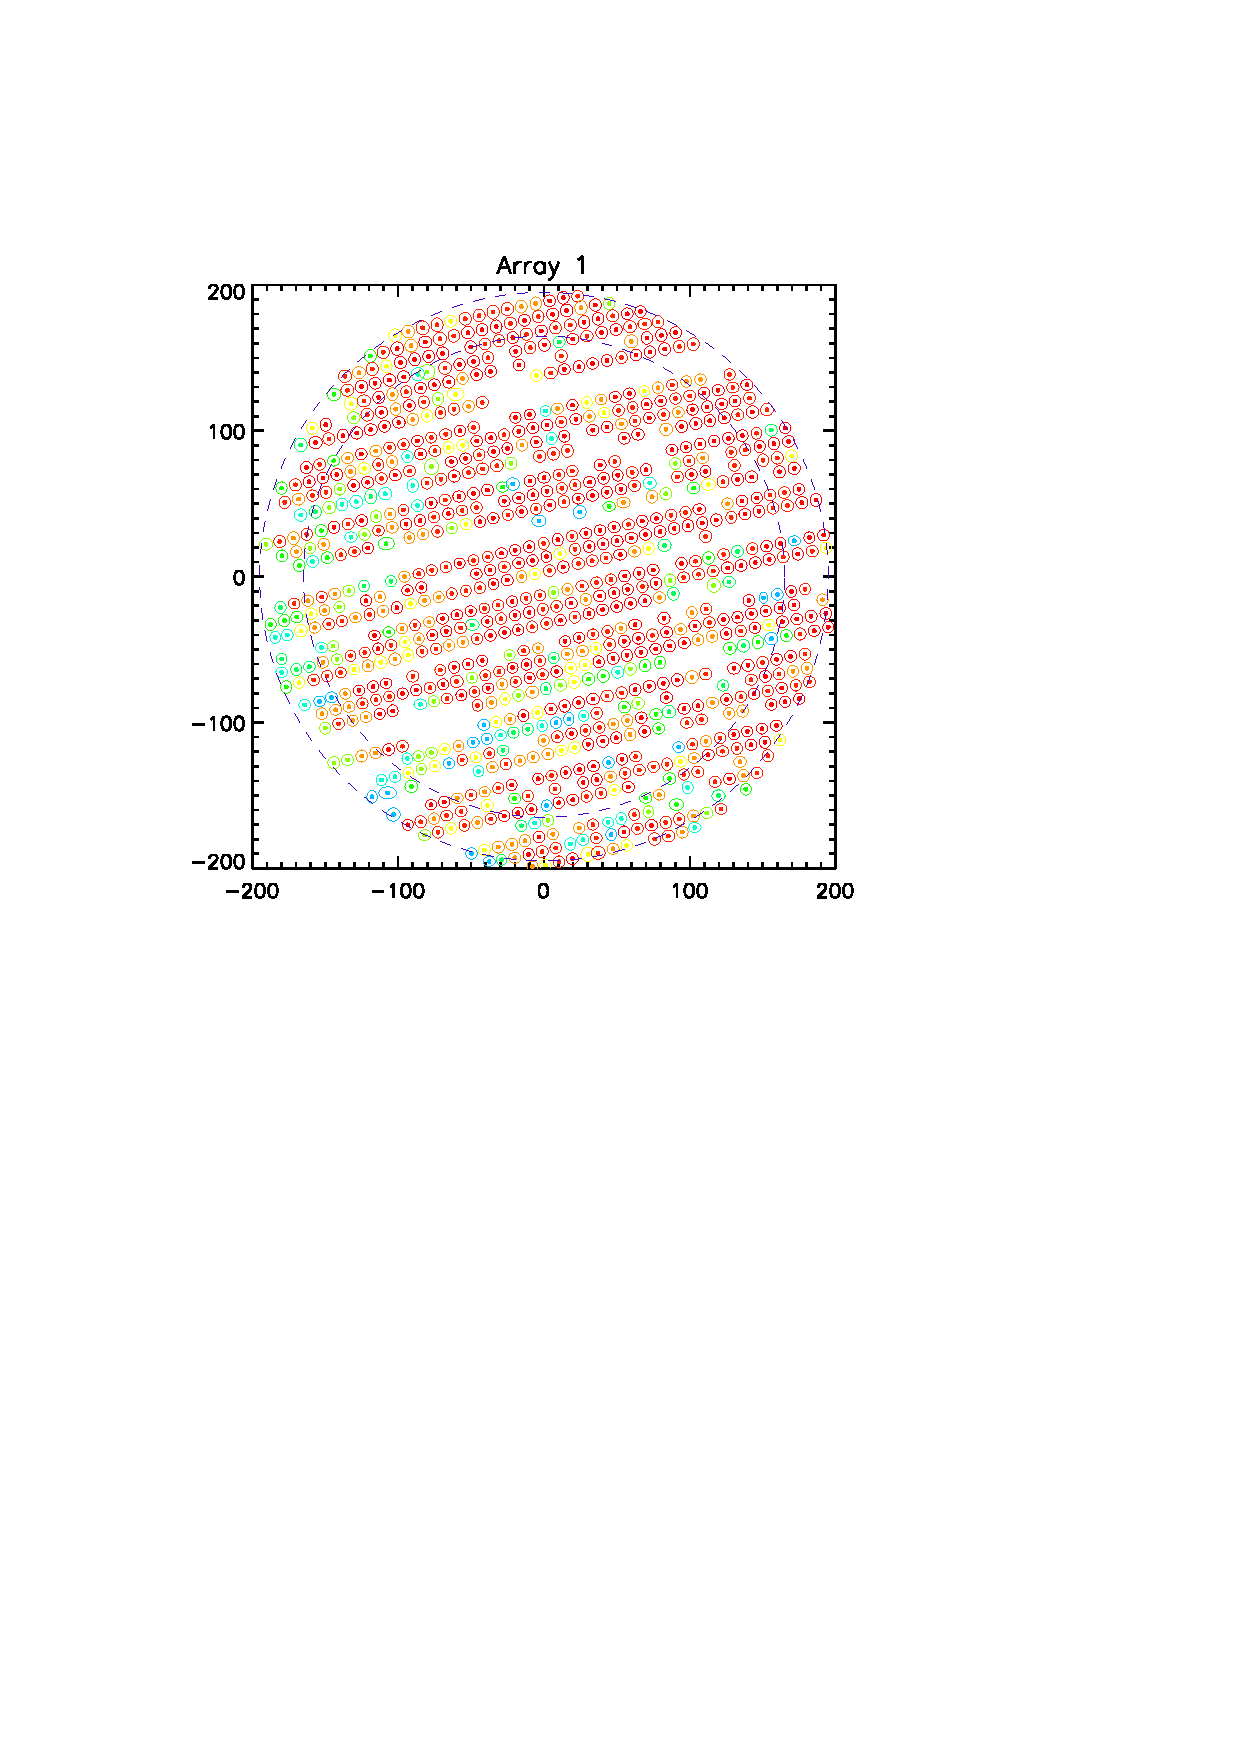
\includegraphics[trim=2cm 14cm 4cm 4cm, clip=true,width=0.45\linewidth]{Figures/A1_fwhm_color_count.pdf}
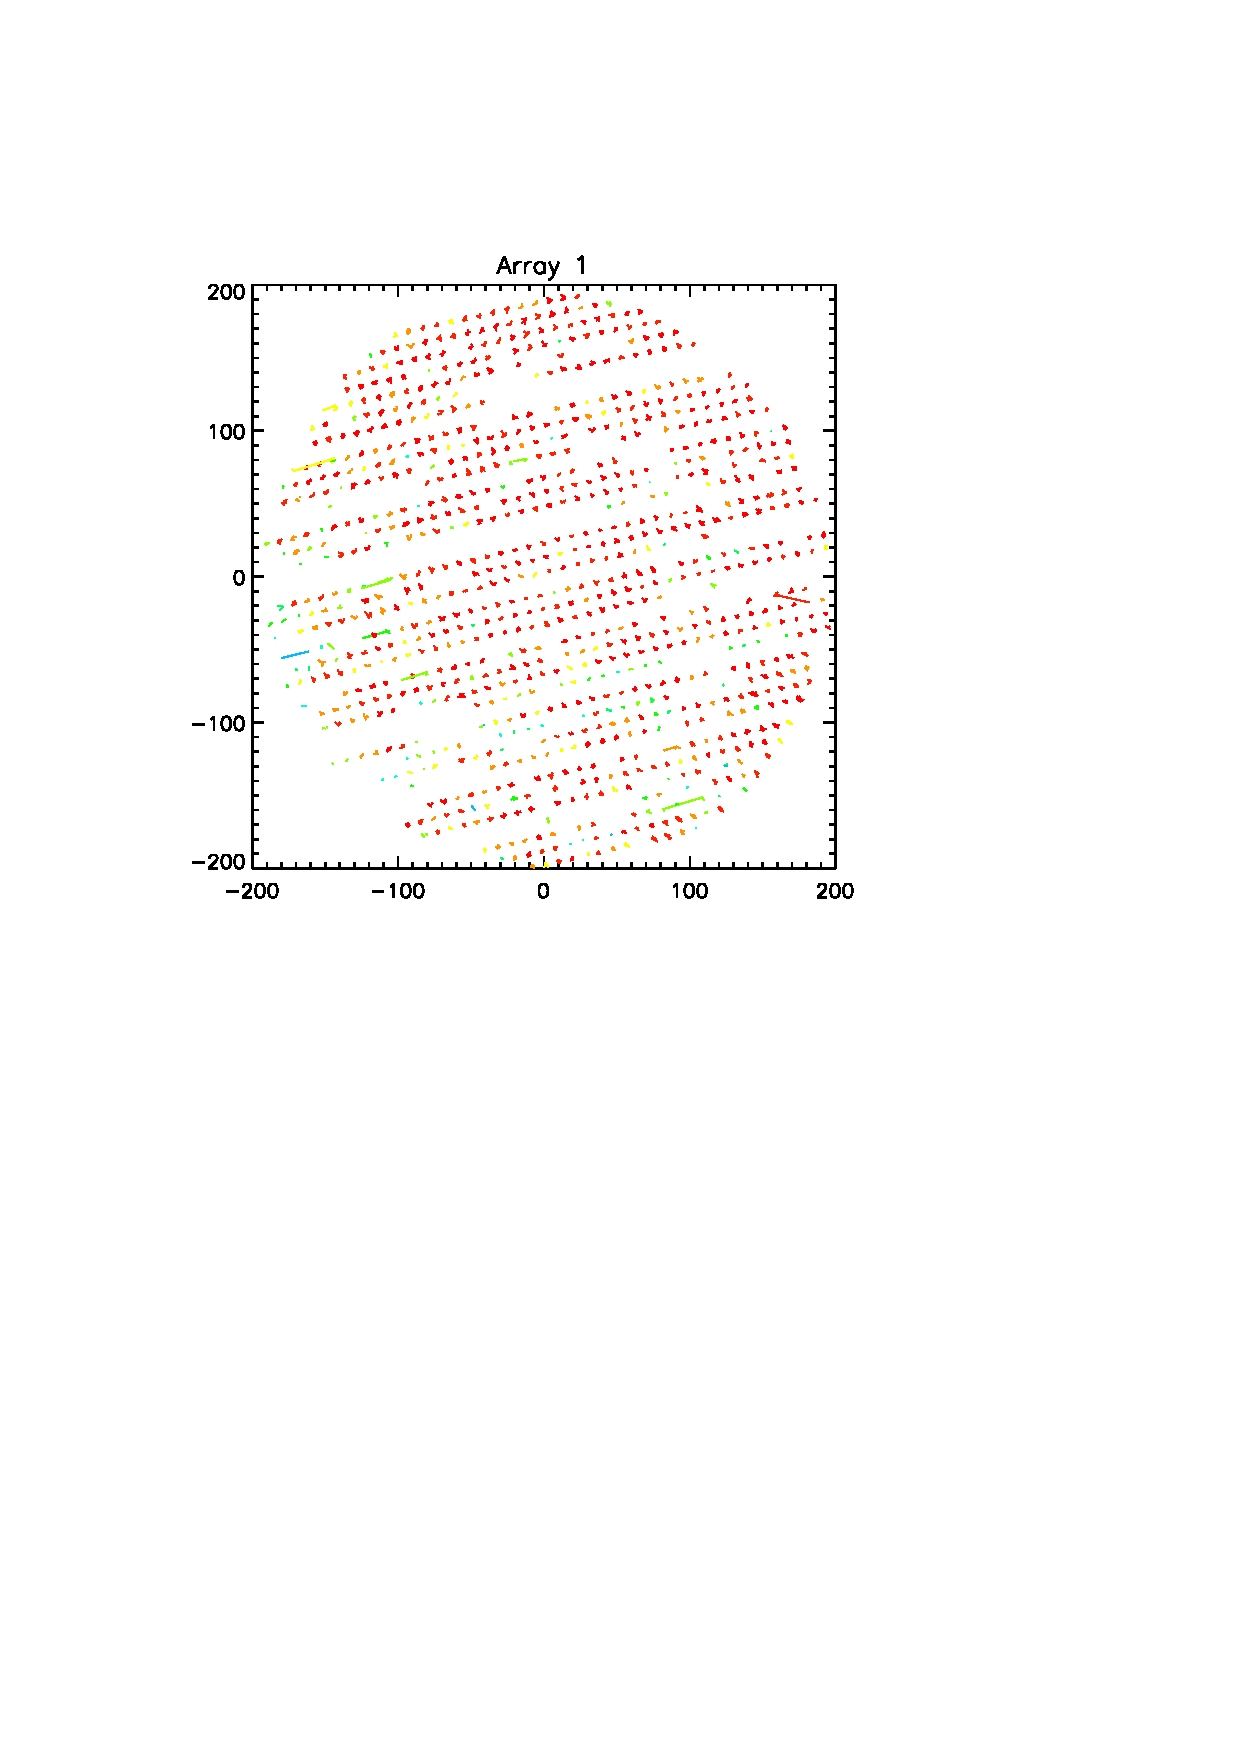
\includegraphics[trim=2cm 14cm 5cm 4cm, clip=true,width=0.45\linewidth]{Figures/A1_positions.pdf}
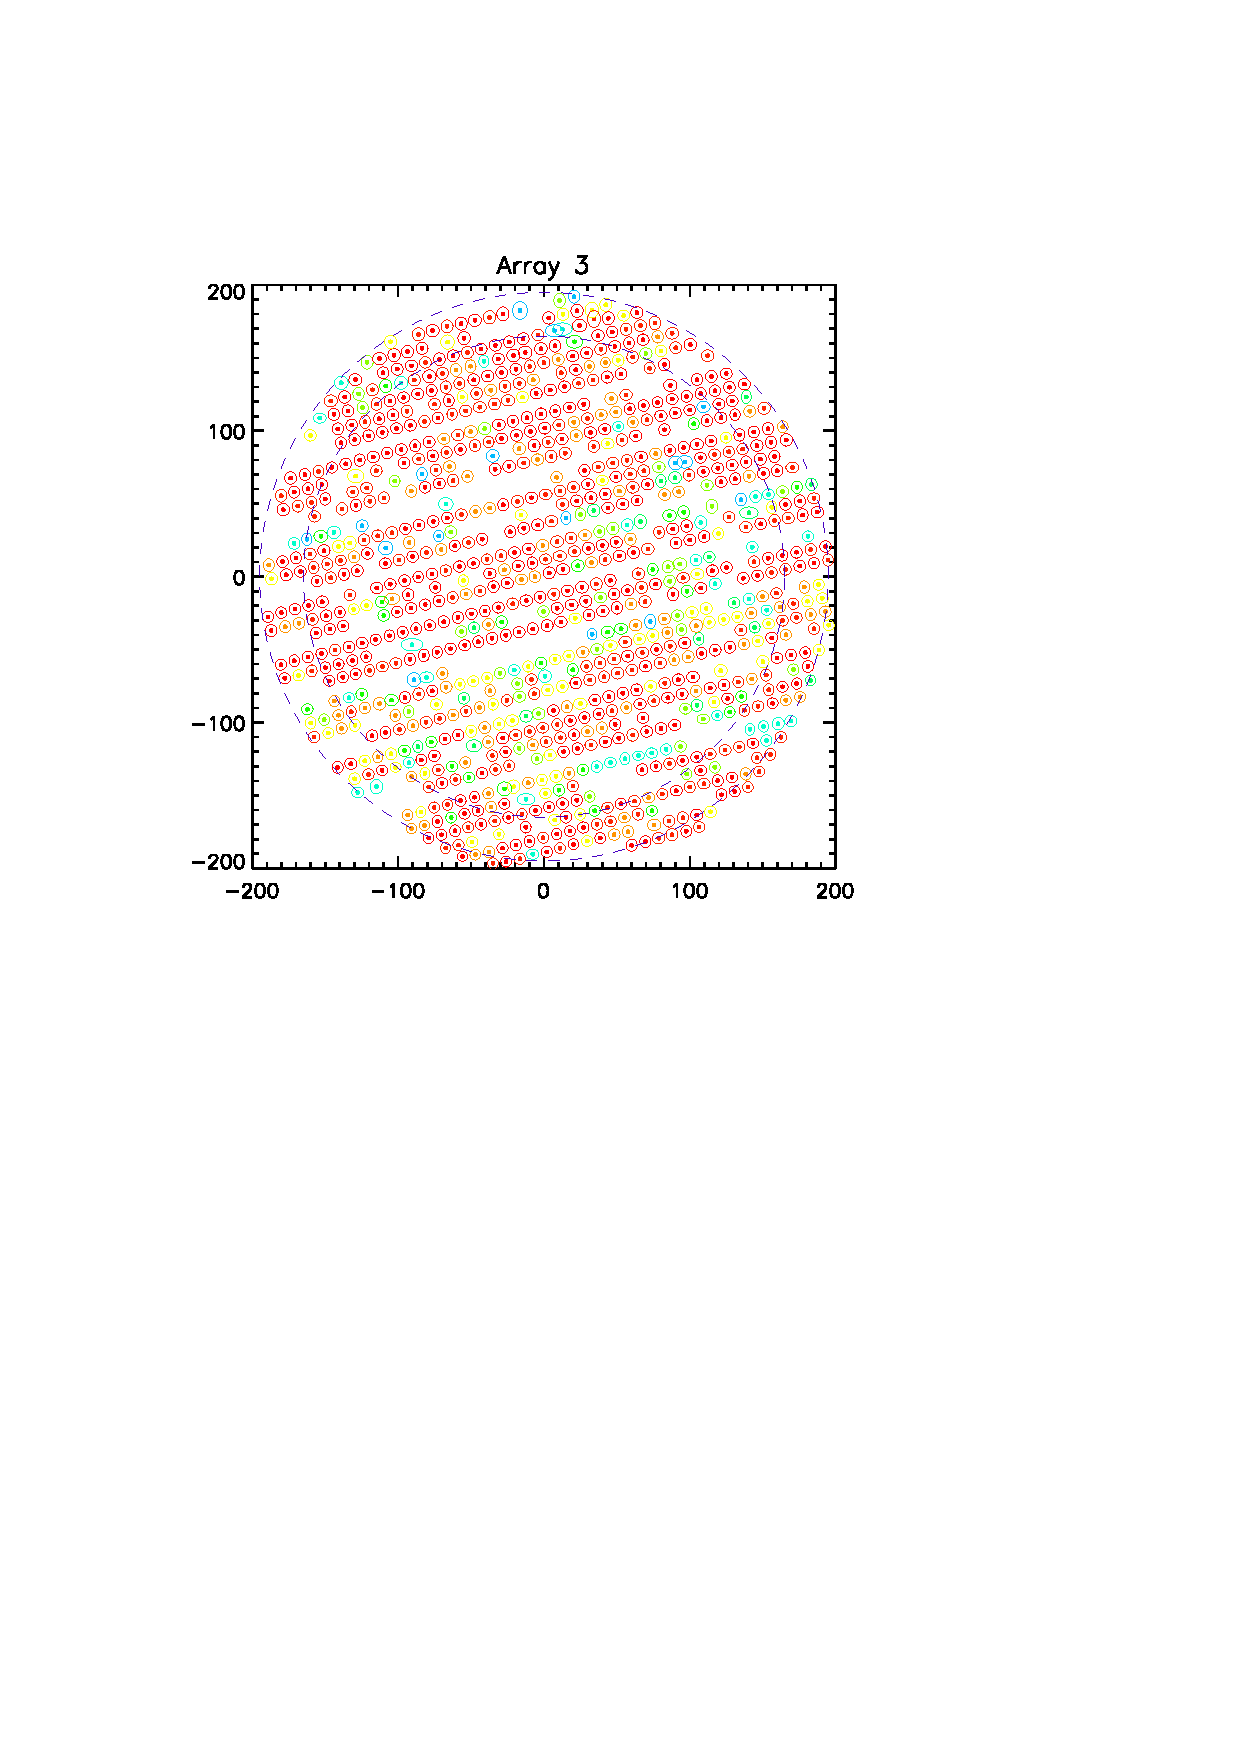
\includegraphics[trim=2cm 14cm 4cm 4cm, clip=true,width=0.45\linewidth]{Figures/A3_fwhm_color_count.pdf}
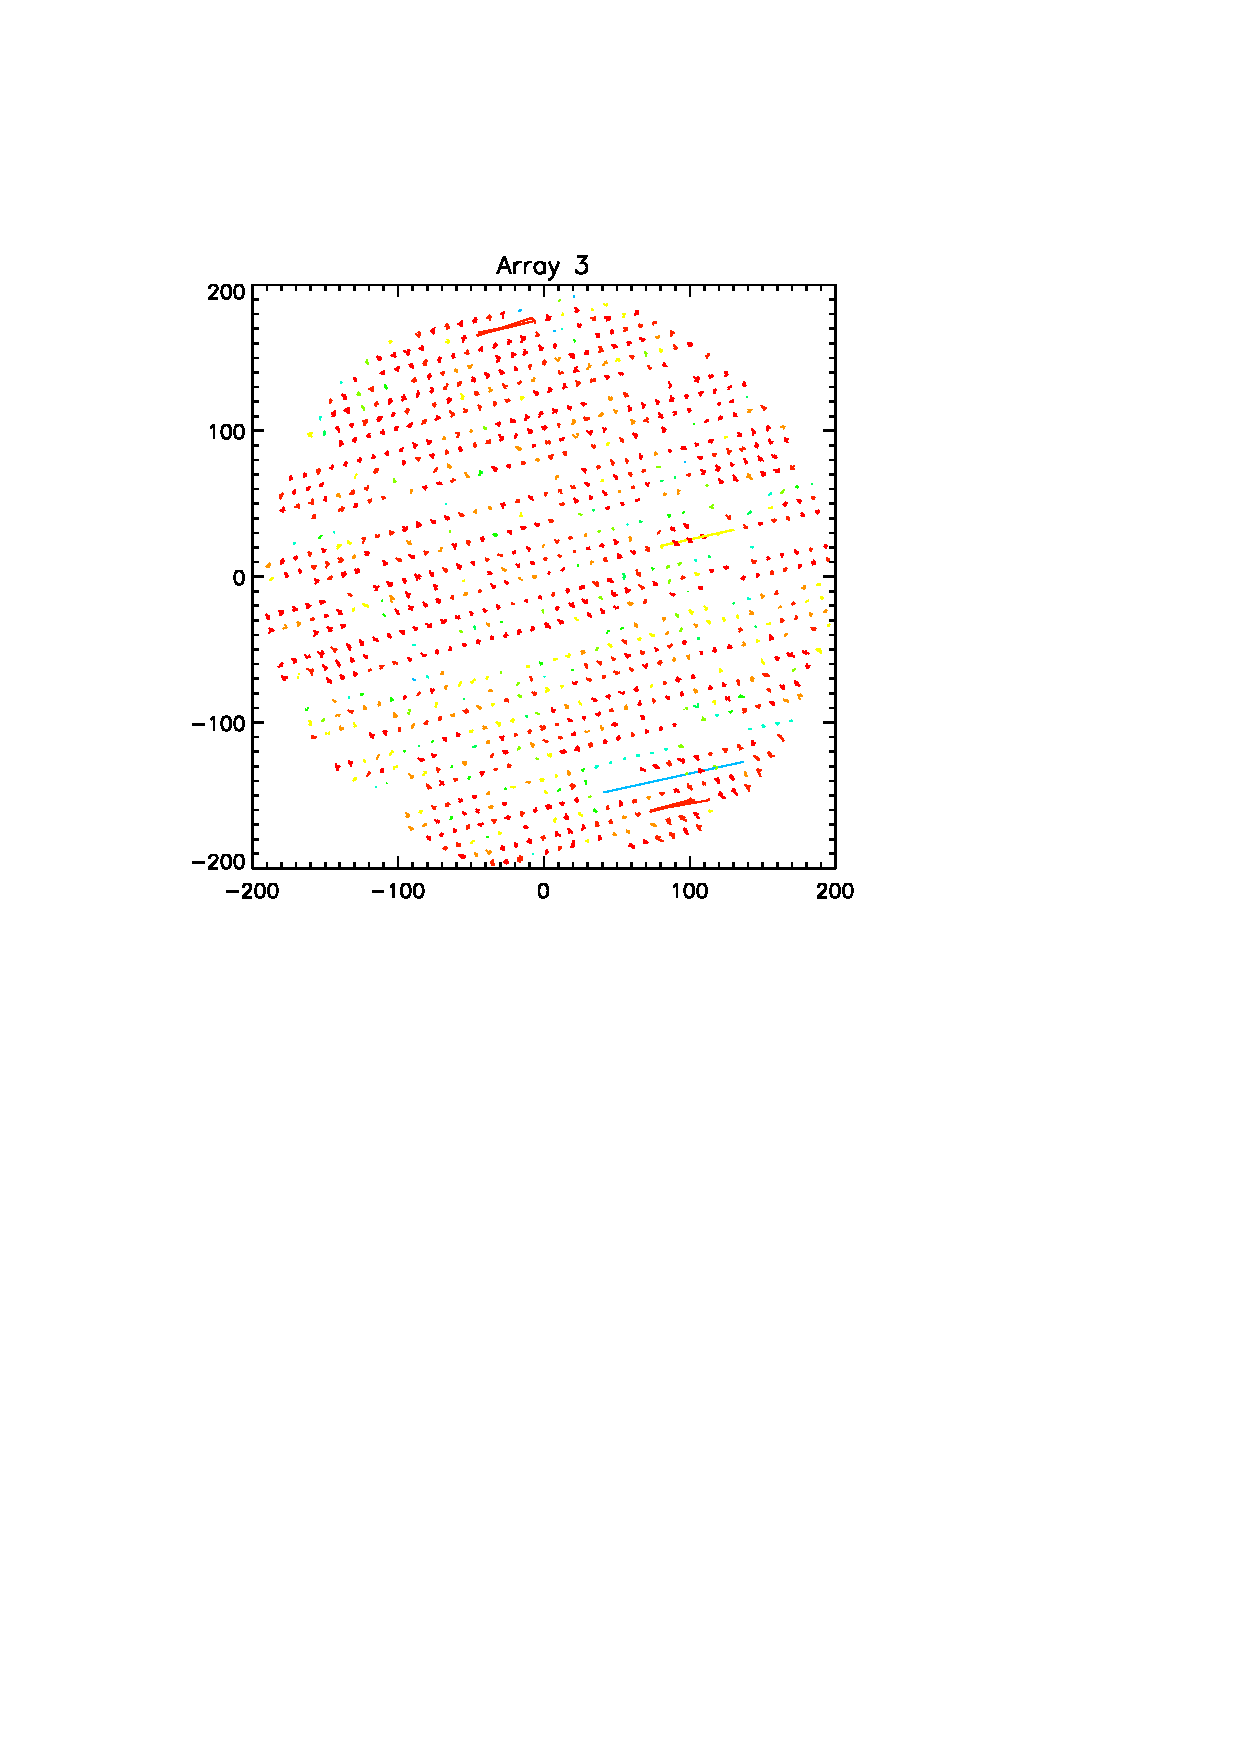
\includegraphics[trim=2cm 14cm 5cm 4cm, clip=true,width=0.45\linewidth]{Figures/A3_positions.pdf}
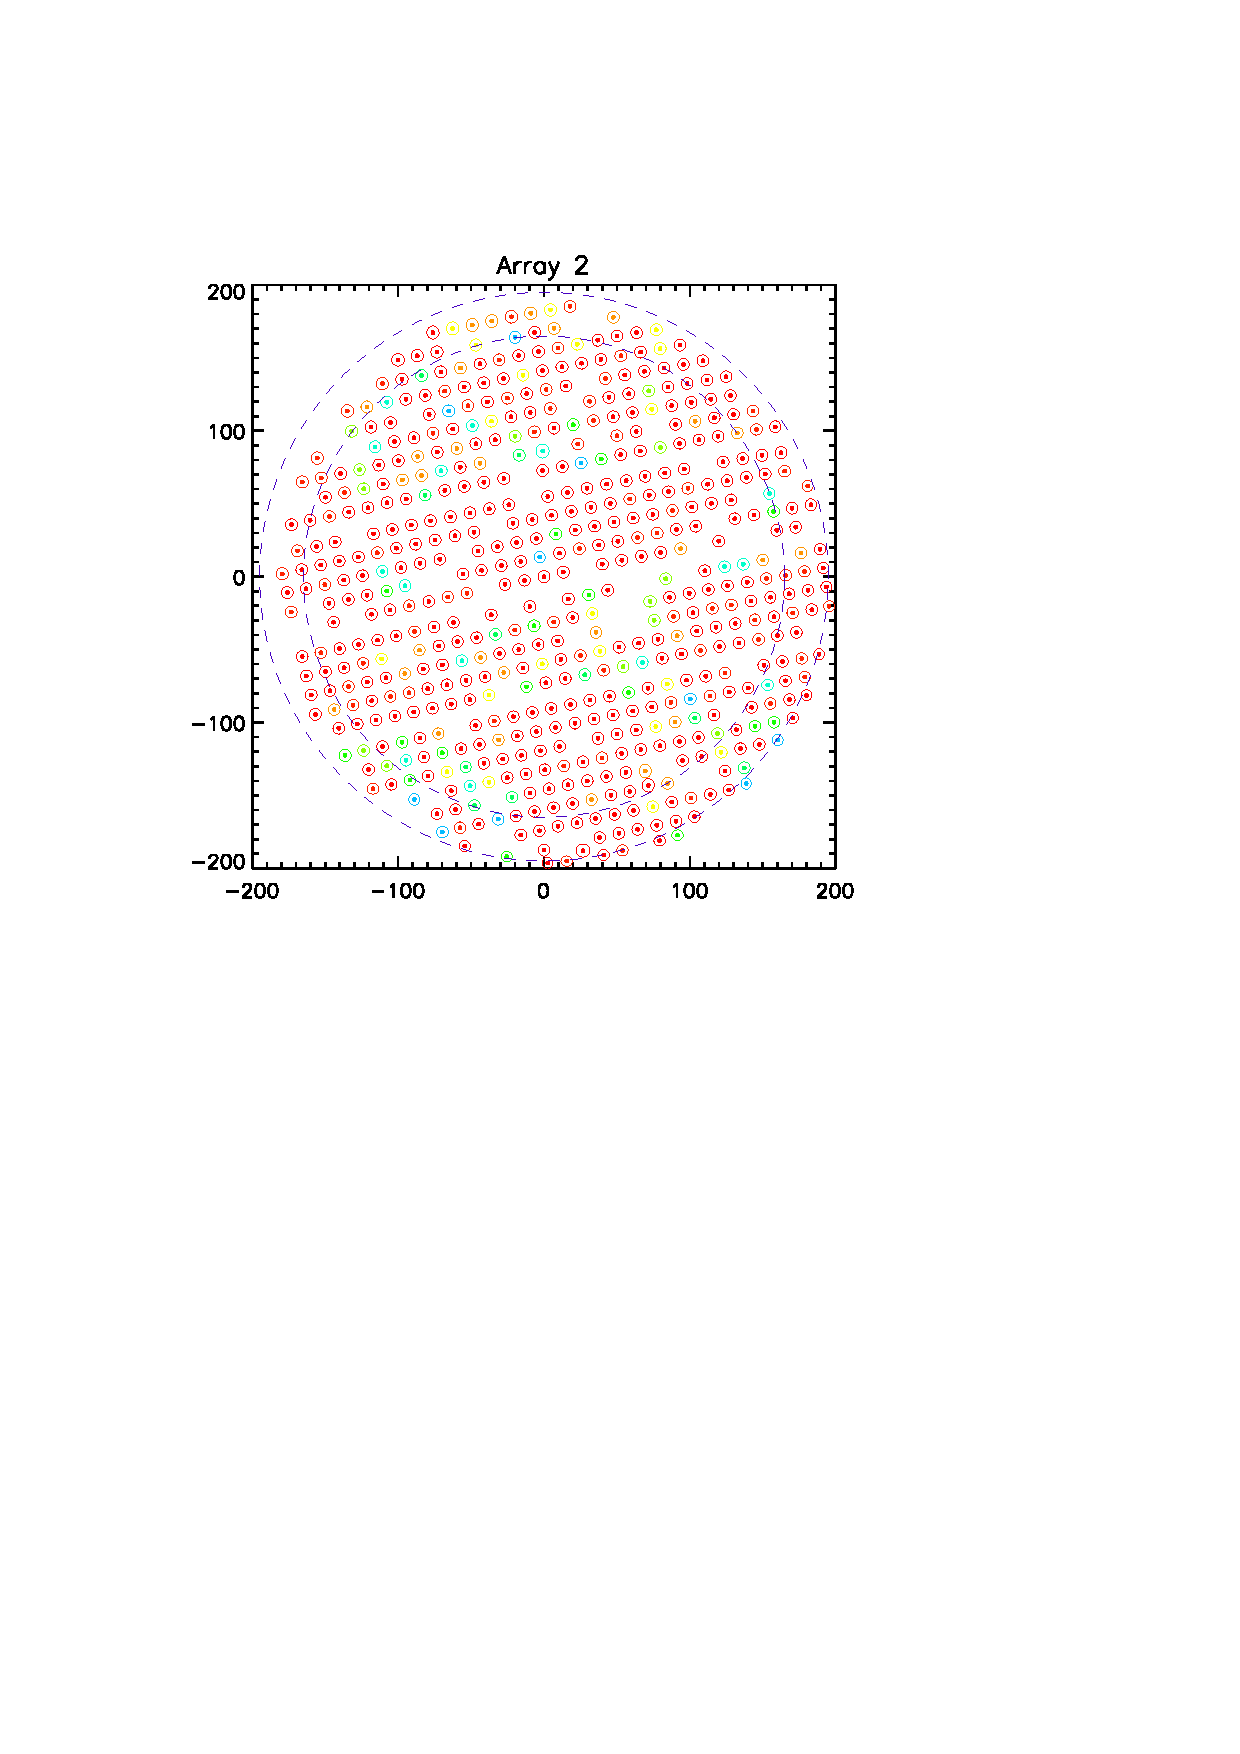
\includegraphics[trim=2cm 14cm 4cm 4cm, clip=true,width=0.45\linewidth]{Figures/A2_fwhm_color_count.pdf}
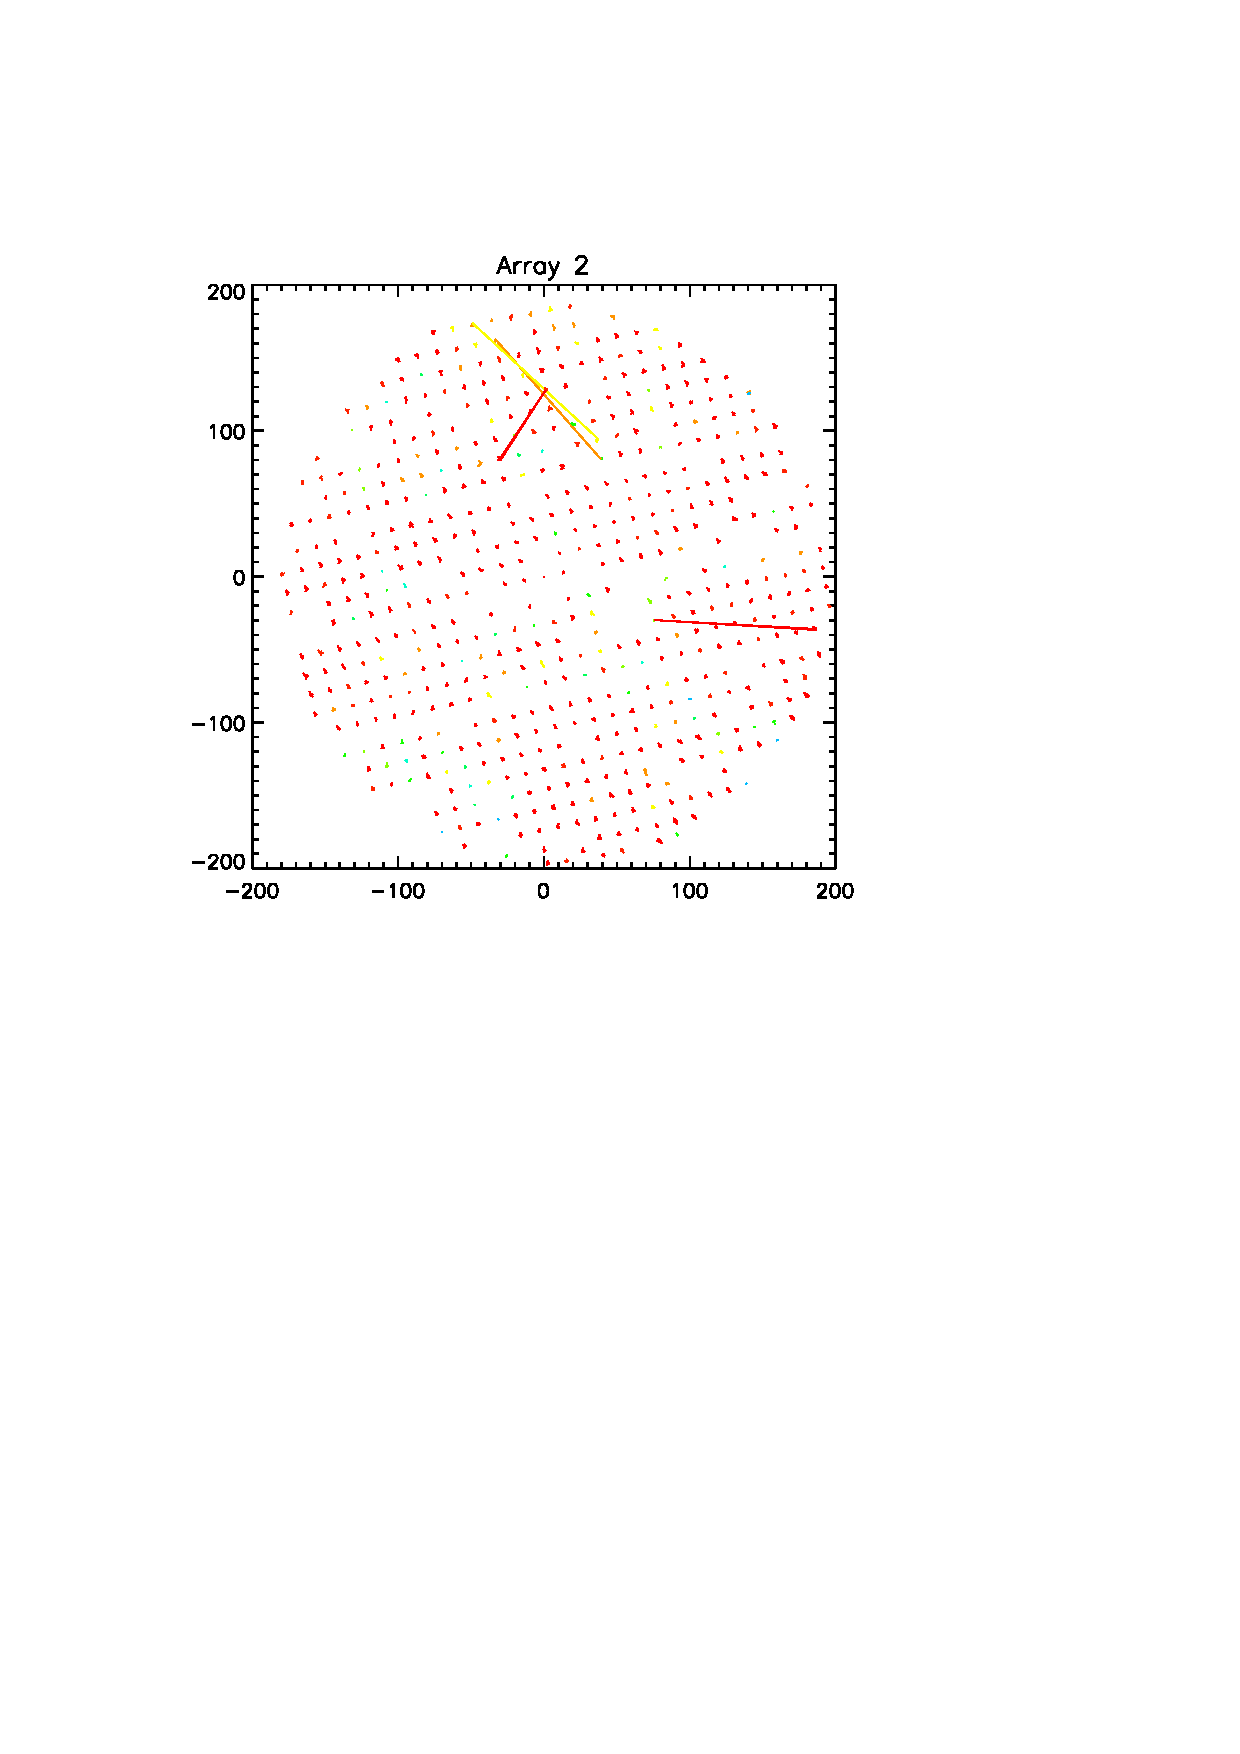
\includegraphics[trim=2cm 14cm 5cm 4cm, clip=true,width=0.45\linewidth]{Figures/A2_positions.pdf}
\caption[KID selection and stability of position in the FOV]{On each of these
  plots, the color indicates, from green to red, how many times a KID was
  identified as valid on a \bm. \emph{Left column:} Average detector positions
  for arrays A1, A3, and A2. The three plots show the detectors that have seen
  the sky and passed the quality criteria for at least two \bms\ during Run10, 9
  and 8: 952, 961, and 553 for A1, A3 and A2, respectively. The inner and outer
  dash-line circles correspond to a FOV of 5.5\,arcmin and 6.5\,arcmin,
  respectively. Units are arcseconds. \emph{Right column:} For valid detectors,
  we show the positions of each pixel, as obtained from each \bm. Some of them
  are not found at the same position for all the \bms\ and are discarded. Units
  are arcseconds.}
\label{fig:avg_fov_color}
\end{center}
\end{figure}

In order to identify the most stable pixels, we compare the KID parameters
obtained with several \bms.  In the following, we show results as obtained using
seven \bms\ from Run10, two from Run9 and one from Run8.  For each pixel we
compute the average position on the focal plane and the average FWHM, counting
the times that it has been considered as valid and at the same position. Indeed,
a few KIDs have close resonances and can be tuned and switched on some scans. A
few others must also be discarded because they appear identical numerically due
to a reminaing artefact in the acquisition. These KIDs are flagged out (less
than 1\% of the designed KIDs). In Fig. \ref{fig:avg_fov_color} we show the
average focal plane reconstruction, from green to red depending on the number of
times that the pixel has been considered as valid. For A1, A3 and A2,
respectively, we have 952, 961, and 553 pixels that have been considered as
valid at least twice (840, 508, 868 valid at least five times). Using this
criterion, we deduce the fraction of valid detectors over the designed ones, as
given in Table~\ref{tab:number_of_kids}.

%% \begin{figure}[htp]
%% \begin{center}
%% 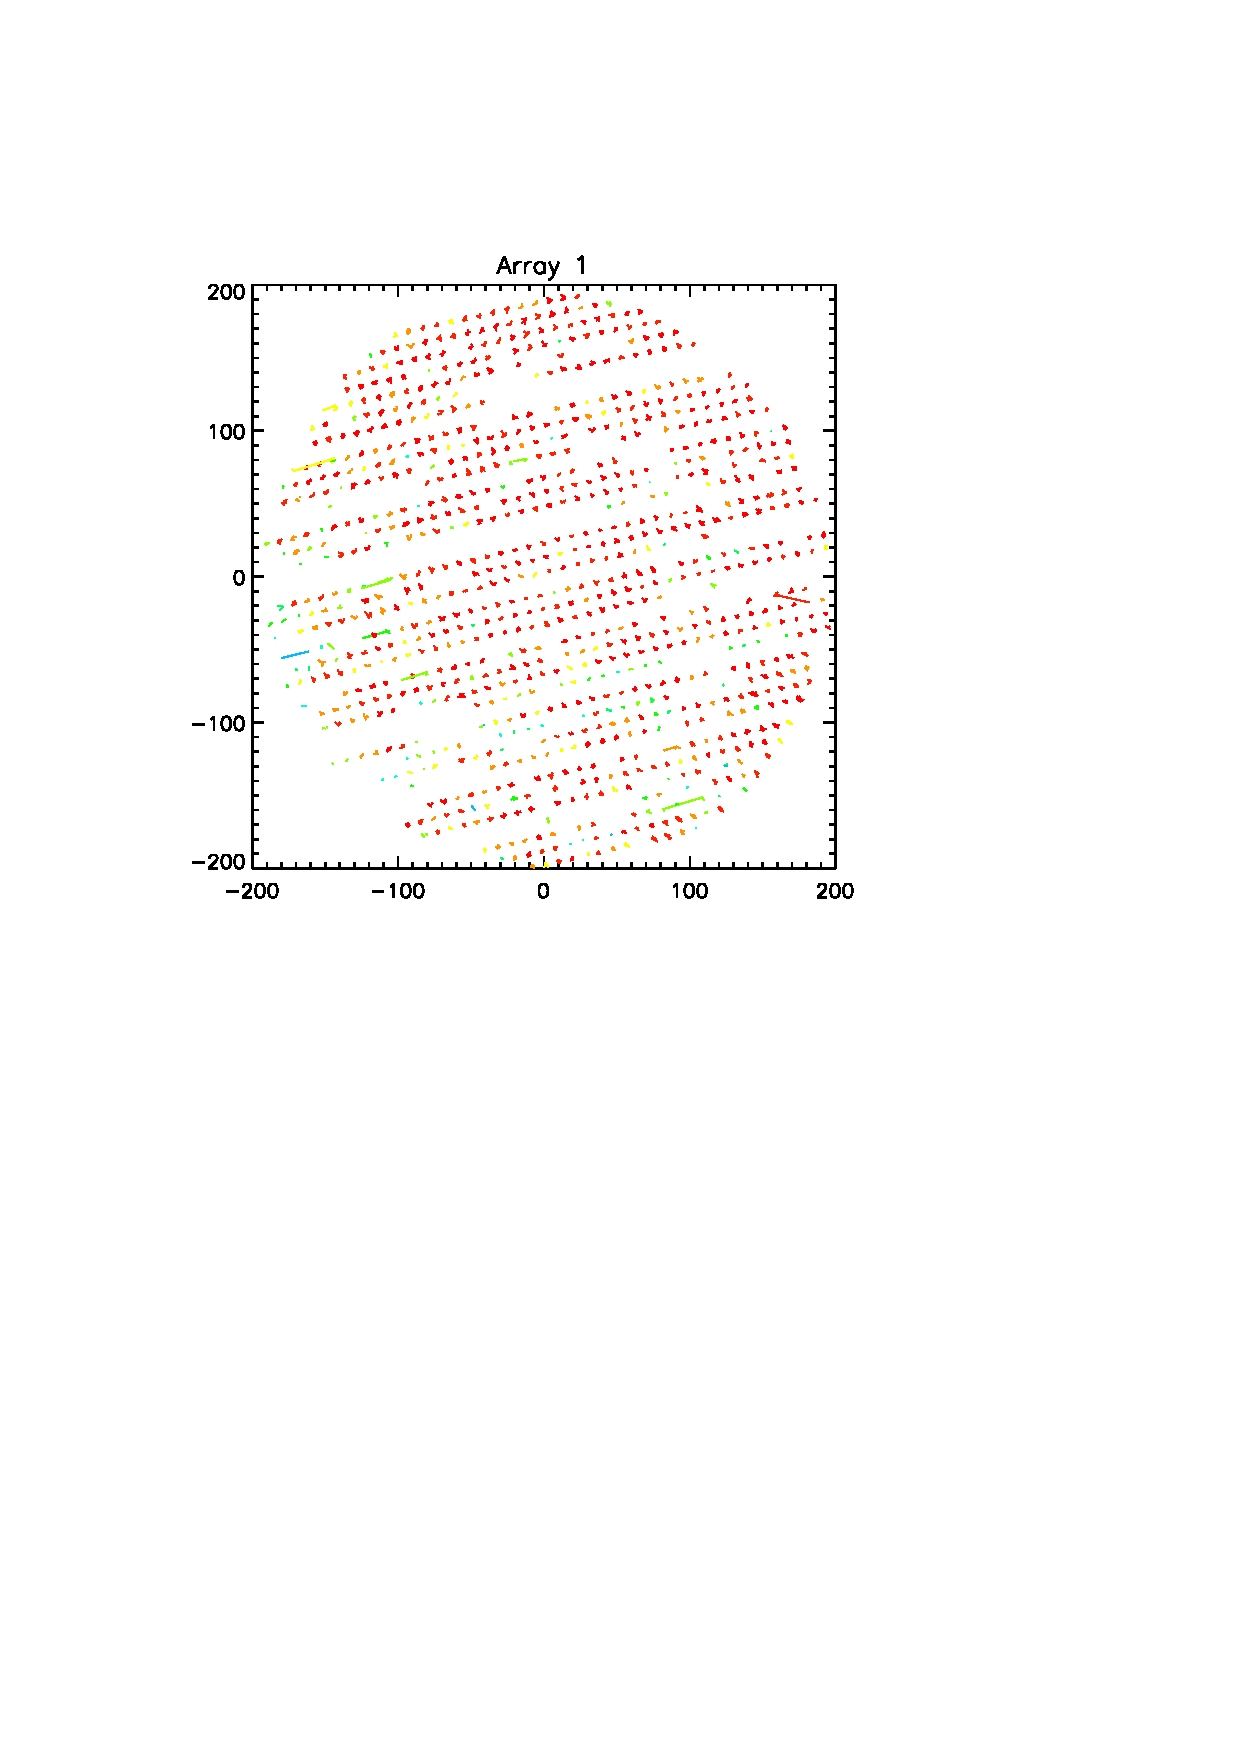
\includegraphics[trim=2cm 14cm 5cm 4cm, clip=true,width=0.55\linewidth]{Figures/A1_positions.pdf}
%% 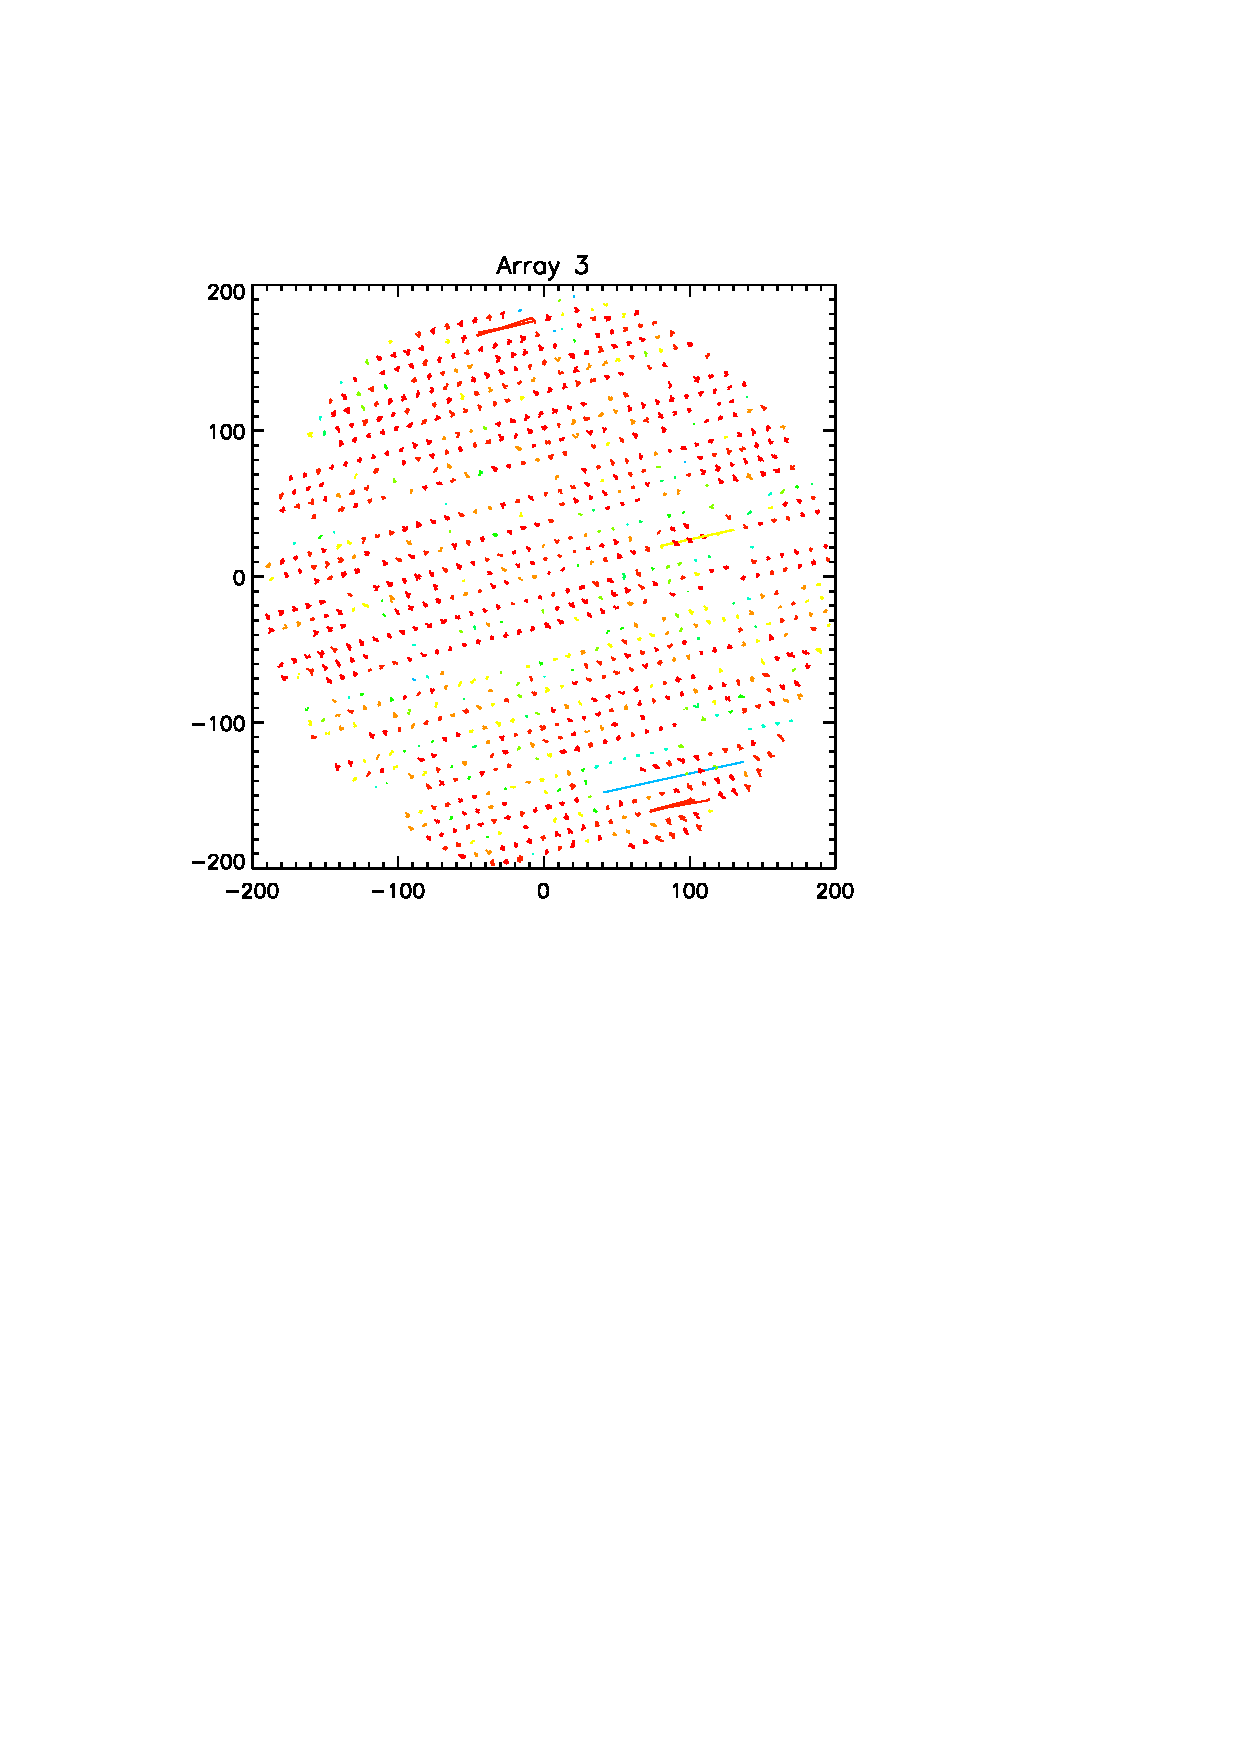
\includegraphics[trim=2cm 14cm 5cm 4cm, clip=true,width=0.55\linewidth]{Figures/A3_positions.pdf}
%% 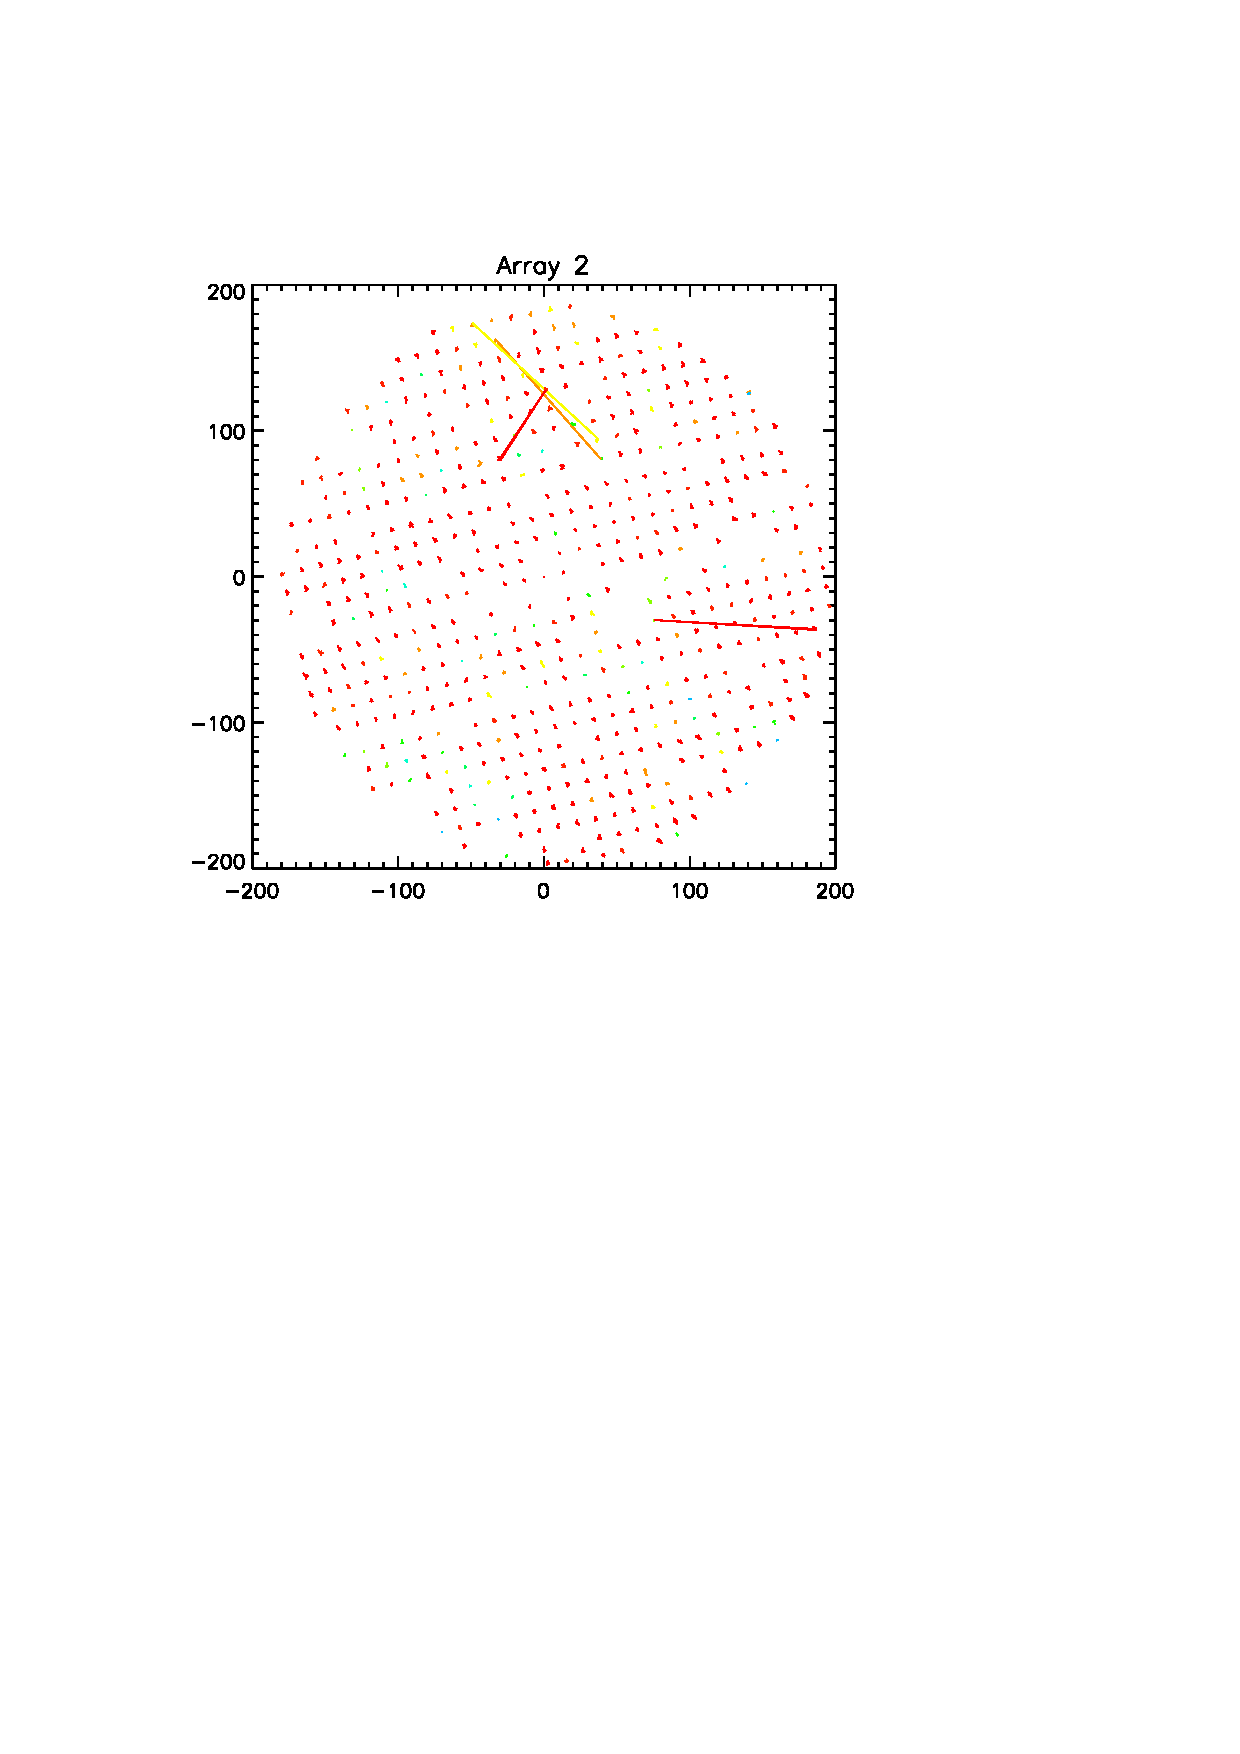
\includegraphics[trim=2cm 14cm 5cm 4cm, clip=true,width=0.55\linewidth]{Figures/A2_positions.pdf}
%% \caption[Stability of KID positions in the field-of-view]{For the valid
%%   detectors, we show the positions of each pixel, as obtained from each beam
%%   map. Some of them are not found at the same position for all the \bms.
%% Units are arcseconds. \todo{{\bf FM : color code : same as on the 1st
%%       maps of validity}}}
%% \label{fig:jumping_kids}
%% \end{center}
%% \end{figure}

%\begin{figure}[htp]
%\begin{center}
%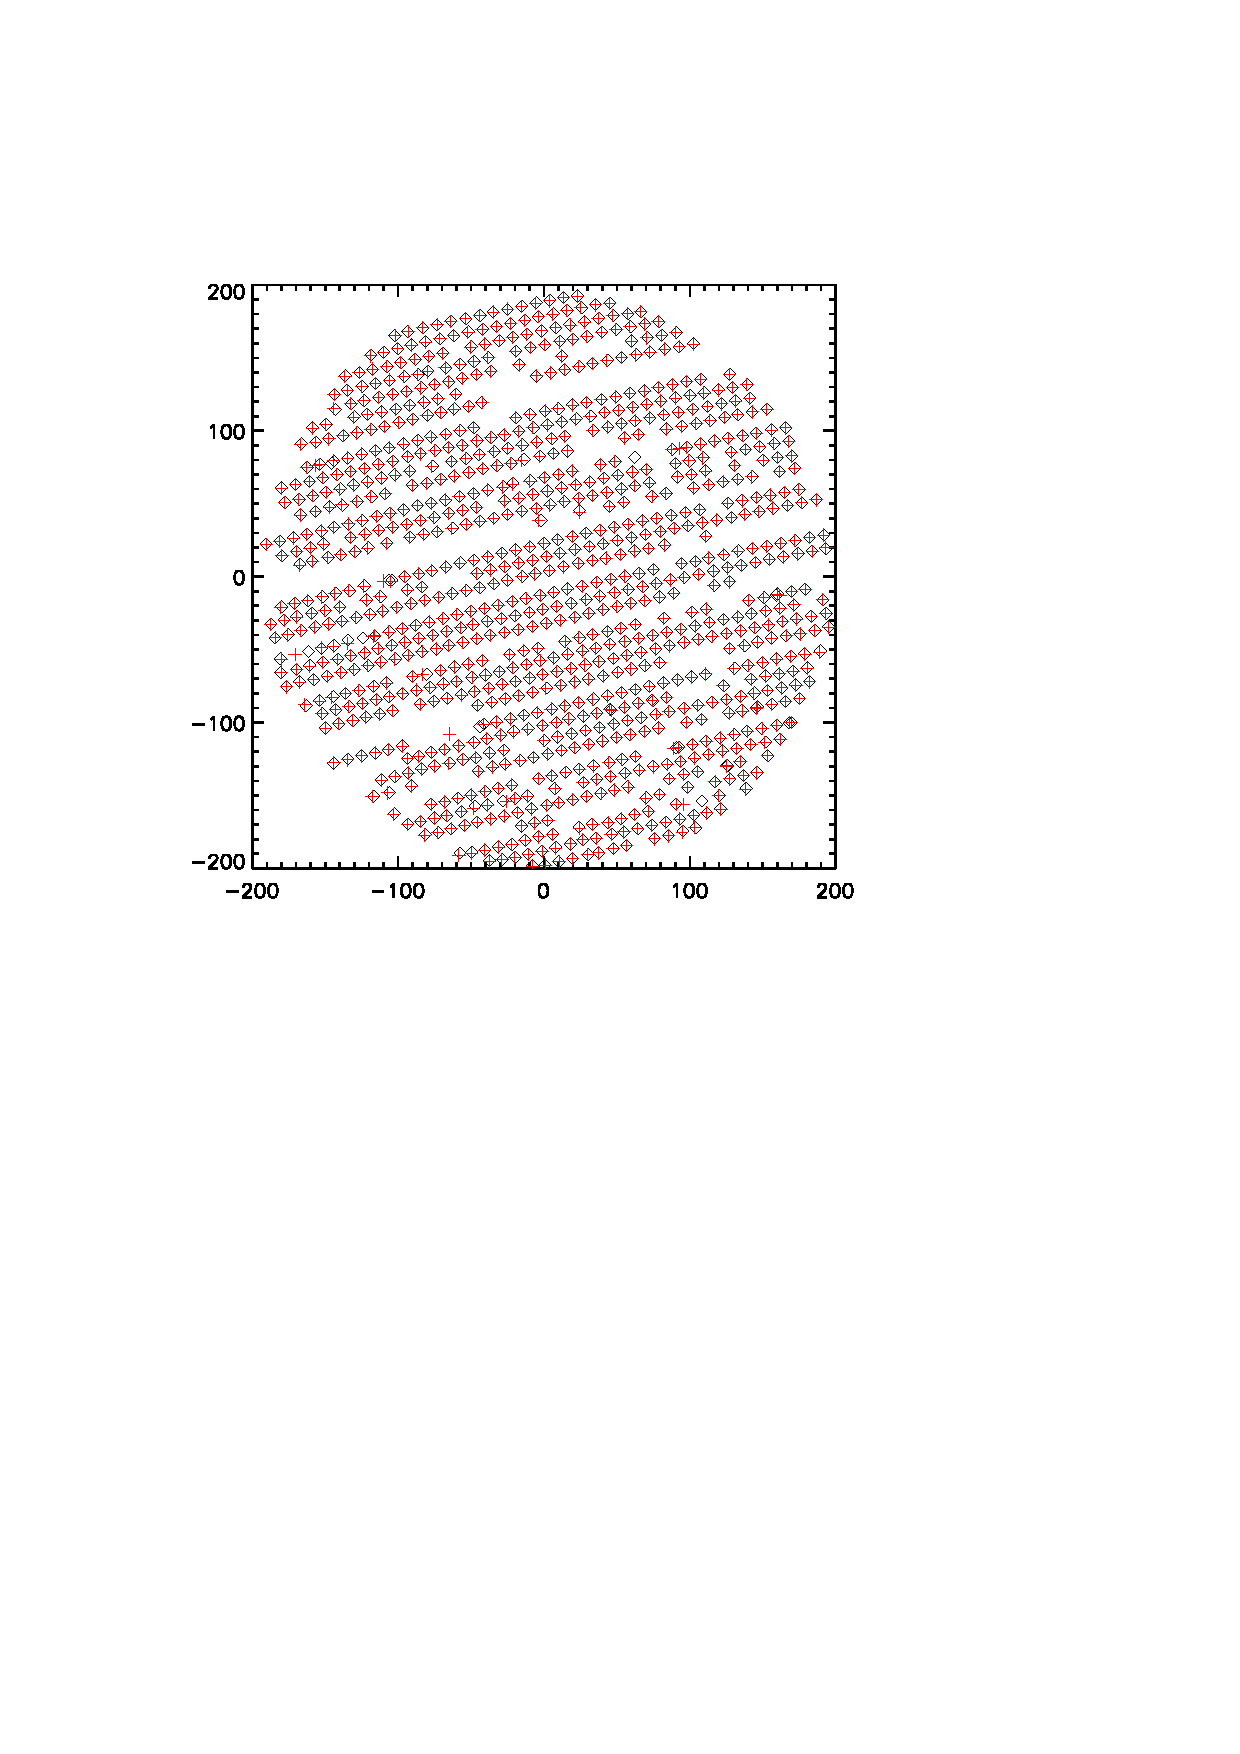
\includegraphics[trim=2cm 14cm 5cm 4cm, clip=true,width=0.55\linewidth]{Figures/A1_test_positions.pdf}
%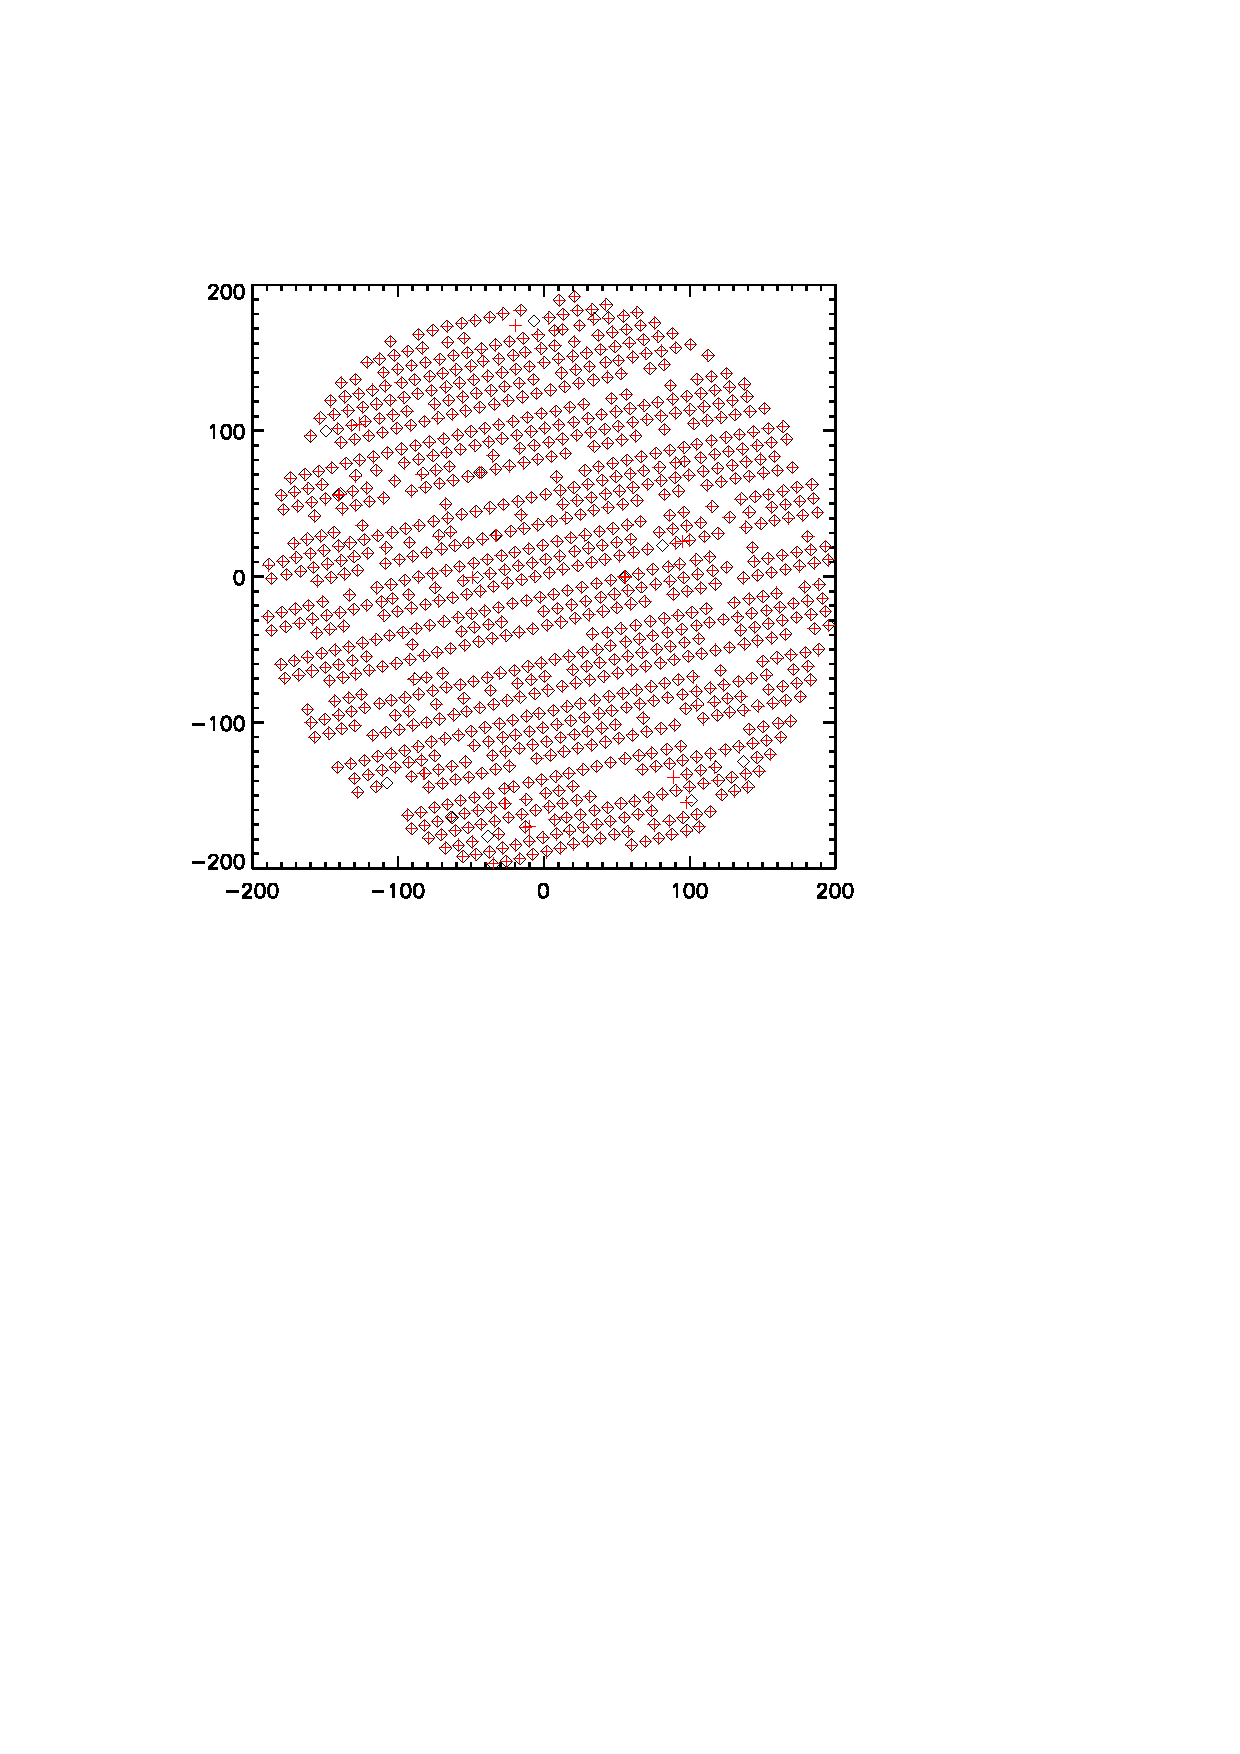
\includegraphics[trim=2cm 14cm 5cm 4cm, clip=true,width=0.55\linewidth]{Figures/A3_test_positions.pdf}
%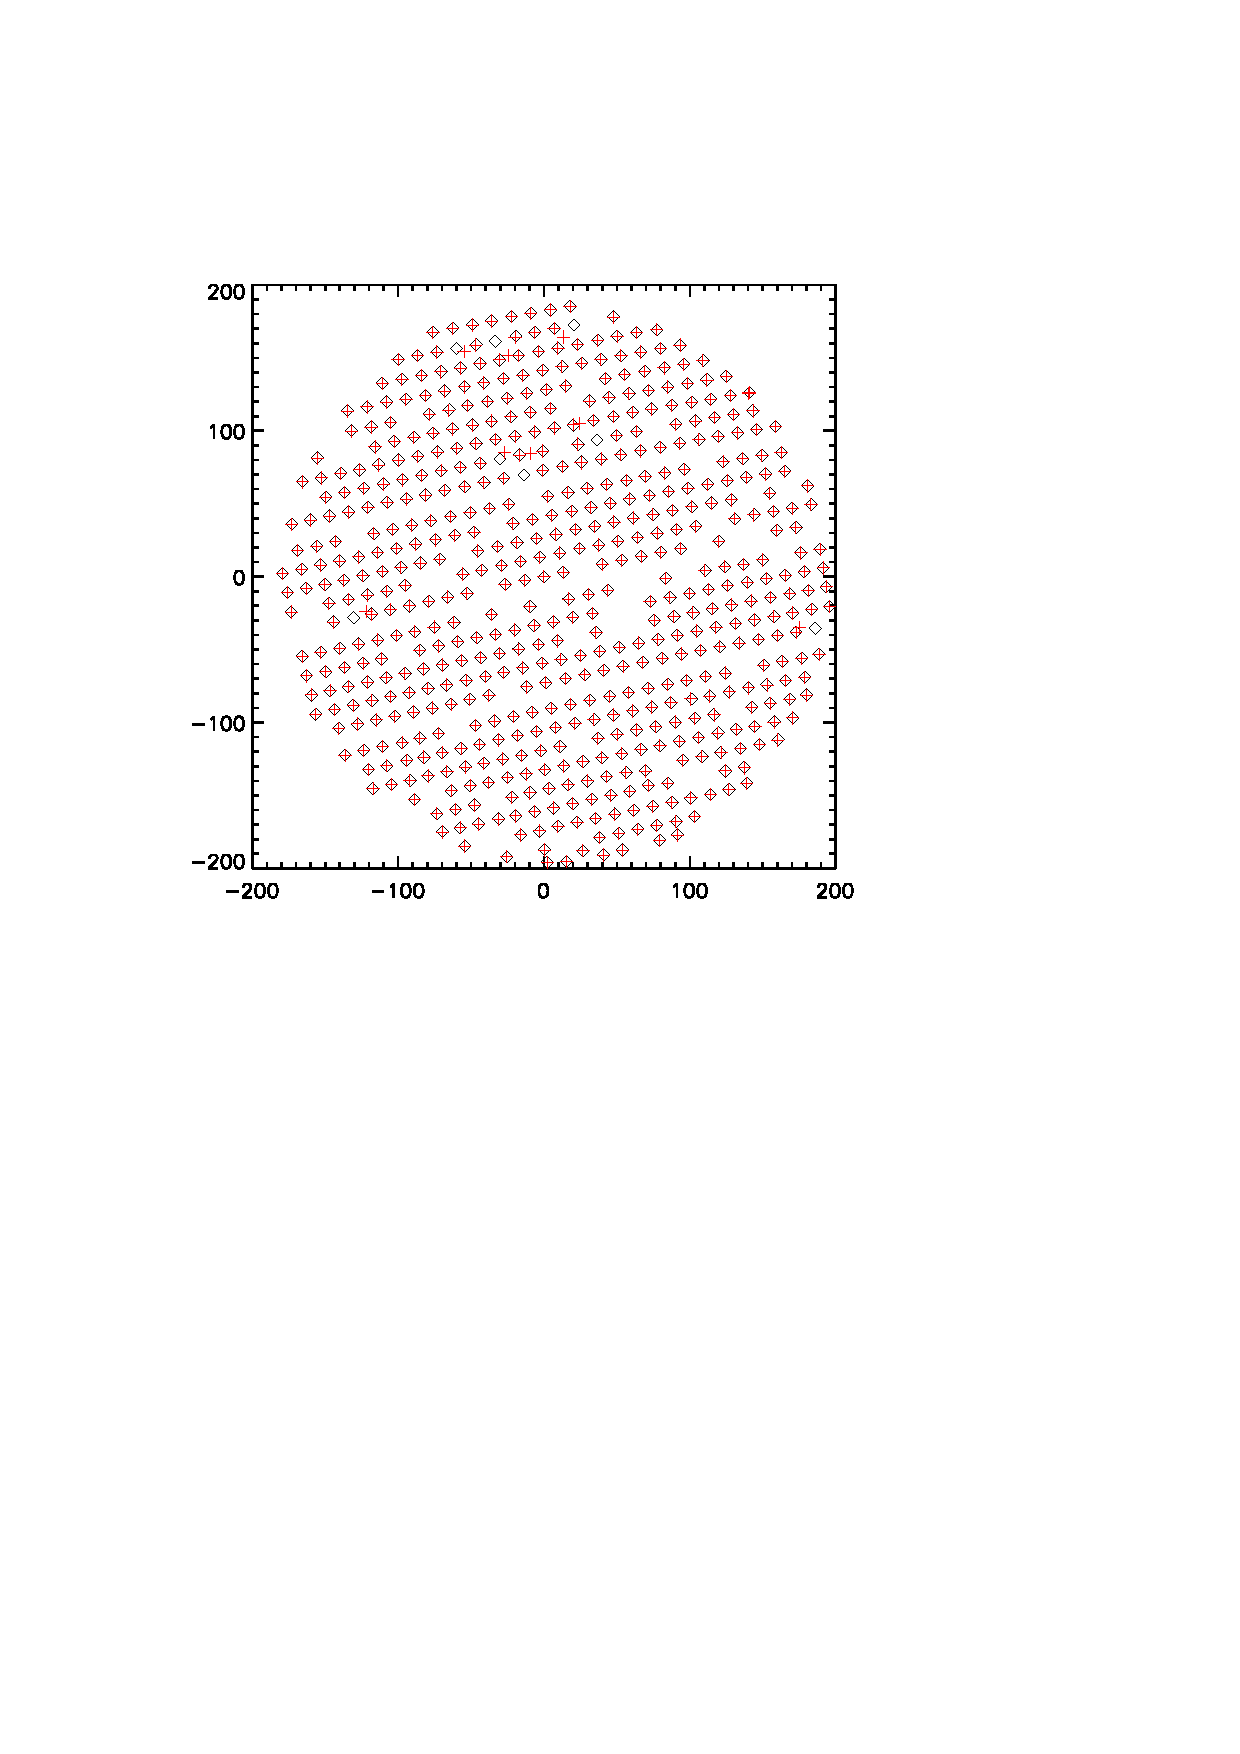
\includegraphics[trim=2cm 14cm 5cm 4cm, clip=true,width=0.55\linewidth]{Figures/A2_test_positions.pdf}
%\caption[Average KID positions]{For the valid detectors,
%  we show the mean (red crosses) and the median (black squares)
%  positions of each pixel, as obtained from each \bm.
%  Units are arcseconds. \todo{FM : color code ? same as on the 1st maps of validity}}
%\label{fig:mean_vs_median}
%\end{center}
%\end{figure}

\begin{table}[ht]
\begin{center}  
  \begin{tabular}{|c|c|c|c|}
    \hline
    Array & Designed detectors &  Valid detectors & Fraction\\
    \hline\hline
    A1 & 1140 & 952 &  84\%\\
    A3 & 1140 & 961 &  84\%\\
    A2 & 616  & 553 &  90\%\\
    \hline
  \end{tabular}
  \caption[Number of detectors]{Summary of the number of valid detectors per array.}
  \label{tab:number_of_kids}
\end{center}    
\end{table}


\section{FOV grid distortion}% {\color{YellowGreen} Xavier }  }
\label{se:grid_distortion}

We studied the matching of the KID position on the sky to the
design position. The global result is scaling, rotation, and shift parameters for each
array. They are described in Table~\ref{ta:gridmatch}.

\begin{table}[ht]
\label{ta:gridmatch}
\begin{center}
\begin{tabular}{|c|c|c|l|}
\hline
Array 1  &	Array 3   &	Array 2   &	Comment \\
\hline
1.25     &      1.25      &     2.05     &     $\lambda$ in mm \\
1140 	 &      1140 	   &        616  &	Total of designed Kids (TDK) \\
673/736  &	734/758  &	437/444  &	Well-placed Kids (WPK)/Found Kids (FK) \\
91/59 	 &    96/64 	 &      98/71 	 & Ratio in [\%] of WPK/FK and WPK/TDK \\
0.87 	 &     0.84 	  & 0.66     &	Median deviation (arcsec) for detectors deviating by less than 5~arcsec. \\
0.52 	 &     0.69 	 &        0.68 	 & Mean distortion across the FoV in arcsec \\
2.3 -4.5  &	2.0 -5.8  &	9.3 -7.5  &	Array center in Nasmyth coordinates (arcsec) \\
4.90  &	4.88  &	4.88  &	Plate scaling (arcsec/mm) in the Design x and y (averaged) \\
77.3  &	76.4  &	78.2  &	Plate rotation angle (degree) from the Design to Nasmyth coordinates \\
6.6  &	6.6  &	6.6  &	FOV [arcmin] (Total kids) \\
9.8/2.00  &	9.7/2.00  &	13.3/2.75  &	Distance between near detectors [arcsec, mm] \\
1.24  &	1.22  &	0.97  &	Distance between near detectors with $30\,\rm{m}$ diameter aperture [in $\lambda$/D] \\
\hline
\end{tabular}
\end{center}
\caption[Field-of-view deformations]{Linear 2D fit of the observed
  position of the detectors in the sky against their mechanically
  designed position for N2R9. The initial table of Found Kids is given
  by the focal plane geometry procedure, as described in
  Sect.~\ref{se:fov_geometry},
  applied to N2R9 \bm\ scans. More than 90\% of the detectors (WPK/FK) are
  within less than 5 arcseconds of their expected position. }
\end{table}

It shows that on average the position of each detector is known to better than
an arcsecond. The 1\,mm arrays have almost the same center but this center
differs by 7 and 2\,arcsec from the 2\,mm array center. The sampling is above
$\lambda/D$ at 1\,mm, assuming a 30\,m diameter aperture. Note that
the plate rotation angle was designed as 76.2\,degrees, less than 2
degrees from what is observed. We find that array 1
has some of the most deviant detectors (above 4\,arcsec from their expected
position). These detectors should be excluded from further analysis. We call
distortion (in the table) the $x.y$ term in the polynomial fitting between the
design grid and the observed position (the fitting is done with the $x$ and
$y$ linear terms and the $x.y$ term). 

This has been compared to expectations obtained using ZEMAX
simulation. The grid diagram generated using ZEMAX provides us with
the maximum dispersion in the field defined by

\begin{equation}
P = \frac{\sqrt{(x_p - x_r)^2 + (y_p - y_r)^2}}{\sqrt{x_p^2 + y_p^2}},
\end{equation}

where $(x_p, y_p)$ and $(x_r, y_r)$ are respectivelly the predicted
and real coordinates on the image surface relative to the reference
field position image location (see page 170 of the ZEMAX manual, 2007).
The predicted coordinates for the whole field are obtained using a
linear interpolation of a small area in the field central part,
whereas the real coordinates are calculated by ray tracing through the
optical system.

\begin{figure}[ht] 
\begin{center}
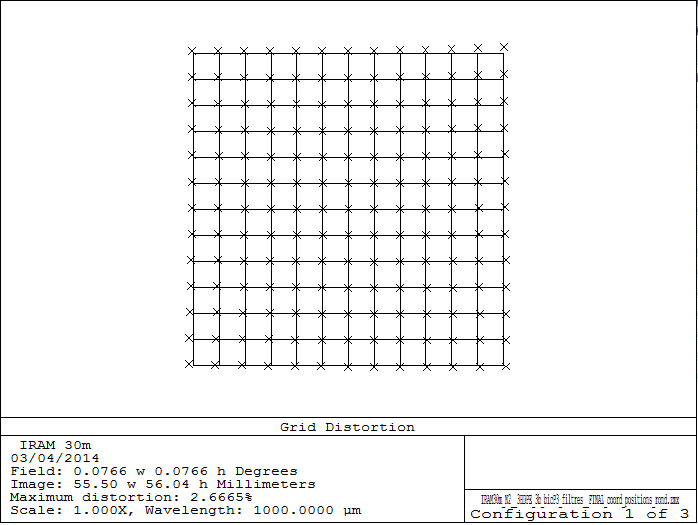
\includegraphics[width=0.9\textwidth]{Figures/NIKA2_Final_grid.png}
\caption[Simulated FOV grid]{NIKA2 grid diagram simulated using ZEMAX. Crosses indicate
  the real coordinates on the Nasmyth image plan. \todo{{\bf question a
    Samuel: pourquoi les dimensions indiquees sont environs 4.5 arcmin
    de cote (et pas 6.5)?}}}
 \label{fig:fov_grid_distortion_zemax}
\end{center}
\end{figure}

Figure \ref{fig:fov_grid_distortion_zemax} show the ZEMAX grid diagram for
NIKA2 simulated optic system. The maximum grid distortion is expected
to be of $2.7\%$ in NIKA2 $6.5'$ FOV. The distortion is the most
noticeable in the upper right corner of the Nasmyth plan, which is
also the area of the largest defocus w.r.t. to the center. 

An expected distortion of $2.7\%$ is at most a 5 arcsecond shift from the
center to the outside of the array.  The quoted measured distortions are not
too dissimilar once the different fitting methods have been taken into
account. Auxillary information on this work can be found in this wiki post\footnote{\tiny
  {\tt http$://$www.iram.fr$/$wiki$/$nika2$/$index.php$/$April$\_$19,$\_$2017,$\_$FXD,$\_$KID$\_$position$\_$mapping$\_$and$\_$Field$\_$distortion$\_$for$\_$Run9}}.

% FXD: this would need to be more ascertained. Lack of time to go further.


%% [Optimal Focus]
%%________________________________________________________
\section{Reconstruction of the focus surfaces}% {\color{YellowGreen} Laurence} }
\label{sec:focus_surfaces}

Owing to the NIKA2 $6.5~\rm{arcmin}$ FOV, the focus is expected to
slightly changes across the FOV, defining curved focal surfaces at the
location of the three arrays. Therefore, beam patterns are expected to
show some scatter across the FOV accordingly to the focal
surfaces. Although all the detectors cannot be individually focalised,
an optimal axial focus of the telescope can be found to maximize the
number of detectors at the best focus and hence, maximize the
resolution of the NIKA2 maps.
This optimal z-focus setting is obtained by measuring the focus at the center of the arrays as described
Sect.~\ref{se:axial_focus} and apply a focus shift, which is primary
predicted using Zemax simulation, and ultimately verified by measuring
the focus surfaces as decribed here.

\begin{figure}
\begin{center}
  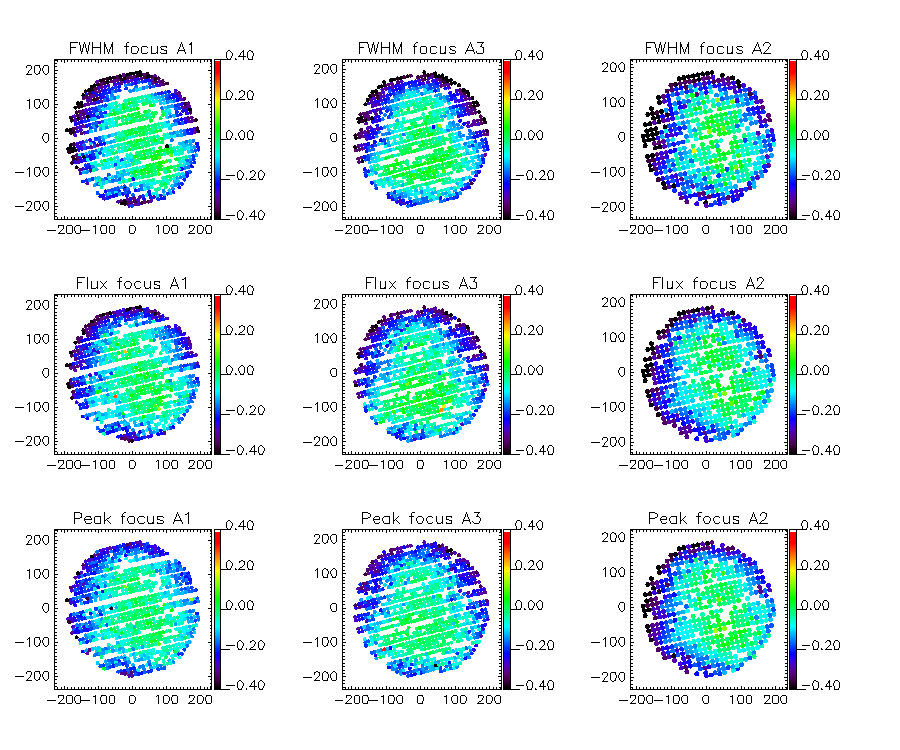
\includegraphics[trim={0, 1cm, 0, 1cm}, clip, angle=0, scale=0.5]{Figures/fov_focus_mv_5.png}
\caption[Focus surfaces]{Focus surface of A1, A3 and A2 arrays from left to
  right. From top to bottom, the focus estimates rely on
  FWHM-minimization, amplitude-maximization of an elliptical
  Gaussian of fixed FWHMs and amplitude-maximization of an elliptical
  Gaussian.}
\label{fig:focus-surfaces}
\end{center}
\end{figure}

\subsection{Method}

We measure NIKA2 focal surfaces by means of a sequence of five
defocused \bms\ of bright
point-like sources, typically Planets or bright quasars, for various settings of
the telescope axial focus around the optimal focus $z_{\rm{opt}}$.
%A \bm\ scan consists of a deep-integrated $13.5' \times 7.8'$ OTF-scan observation
%comprizing $99$ sub-scans and with a scanning speed of either $65''/s$ whenever
%the mean integration elevation is $< 60$ degree or $39"/s$ at higher
%elevation.
The z-focus is changed in step of $0.6~\rm{mm}$ to probe a large
focus range for measuring even the extreme variation of the focus surfaces,
namely $z \in \{-1.2, -0.6, 0, 0.6, 1.2 \} + z_{\rm{opt}}$.  Each
\bm\ are analysed using the data reduction pipeline, as described in
Sect.~\ref{se:pipeline_overview}, and $4''$-resolution individual maps per kid
are projected. %Before the projection, the correlated noise is mitigated from each KID timeline in
%subtrating out a common mode, which is obtained using, amongst the other
%detectors, those that correlates the most with this KID and that are located
%outside a radius of $90''$ around the source centroid.
Therefore, a series of
five cleaned maps at various focus is available for each detector, from which
the best focus is estimated as described in Sect.~\ref{se:axial_focus}. The
ensemble of the relative focus estimate per KIDs with respect to the best focus
at the center of the array constitutes the focus surface. An accurate estimate
of the center focus is obtained as the weighted average focus estimate of the
KIDs lying in a $30''$ radius around the geometrical center of the array. This
average does not induce any sizeable bias thanks to the flatness of the focus
surface in the innermost regions. For robustness test, we consider three focus
estimates: the two first ones are the same as discussed in
Sect.~\ref{se:axial_focus} -- namely i) $\hat z_{\rm{fwhm}}$ the focus that
minimizes the geometrical FWHM and ii) $\hat z_{\rm{peak}}$ the focus that
maximizes the amplitude of the best-fitting ellitical Gaussian -- whereas the
third one is $\hat z_{\rm{flux}}$ the focus that maximizes the amplitude of the
best-fitting elliptical Gaussian of fixed FWHM (at $12.5''$ at $260~\rm{GHz}$ and
$18.5''$ at $150~\rm{GHz}$). The comparison between the two amplitude-based
estimators ($\hat z_{\rm{peak}}$ and $\hat z_{\rm{flux}}$), will test the
stability of the focus results against the exact choice of the beam fitting
function. Since the ellipticity-based estimator $\hat z_{\rm{ellip}}$ is less
sensitive to focus changes and yields larger uncertainties than the others, we
do not use it for the focus surface reconstruction.


\subsection{Data set}

After the change of A1 lens and the improvement of internal optics
alignment (hence in the final NIKA2 optic configuration) that is
during the N2R8 two-day run, N2R9 and N2R10,   
nine defocused \bm\ sequences have been acquired, including incomplete
sequences and sequences hindered by poor atmospheric conditions.
We select sequences that i) comprises at least four scans, ii) have been
observed at zenith opacity at $225~\rm{GHz}$ (as indicated by
the IRAM taumeter) below 0.5 and iii) have a maximal central focus
drift between the starting time and the end of the sequence of
$0.5~\rm{mm}$. These criteria preserve five sequences from which focus
surfaces can be reconstructed. Namely, we consider the sequences
$20170226s415\mbox{--}419$, $20170419s133\mbox{--}137$, $20170420s113\mbox{--}117$,
$20170421s160\mbox{--}164$ and $20170424s123\mbox{--}127$, which consist of observations
of the bright quasar 3C84 and Neptune.

\subsection{Results}
For each detector $k$ and each \bm\ sequence $s$, we obtain for
the array $a$, a focus measurement $z_k^{a, s} \pm \sigma_k^{a, s}$,
where $\sigma_k^{a, s}$ is the $1\mbox{--}\sigma$ error of the least-square
polynomial fit. The focus surface measurements per array obtained from the five
\bm sequences are combined using an inverse-variance weighting
scheme to obtain the focus surface estimates 
\begin{equation}
\label{eq:mv_focus_surf}
z_k^{(a)} = \left( \sigma_k^{(a)} \right)^2 \,  \sum_s \frac{z_k^{a,s}}{\left(\sigma_k^{a,s}\right)^2}\, \,  ,
\end{equation}
with uncertainties 
\begin{equation}
\label{eq:error_mv_focus_surf}
\sigma_k^{(a)} = \left[ \sum_s \frac{1}{\left(\sigma_k^{a,s}\right)^2}\right]^{-1/2}\, .
\end{equation}


We present NIKA2 focus surfaces per array obtained as in
Eq.~\ref{eq:mv_focus_surf} 
%from the inverse-variance weighted combination of the five
%reconstructed focus surfaces per arrays
in Fig.~\ref{fig:focus-surfaces}.
The three flavours of focus-estimators provide us with focus surfaces
per array that are in good agreement with each others and that have a
non-axisymetrical flatten bowl shape consistent with expectations from
optic simulation. %{\bf [TBA, as discussed further below]}.
The median defocus (that is the relative focus w.r.t. the center)
across the detectors is about
$-0.1~\rm{mm}$ for the three arrays. Maximal defocus values of about
$-0.6~\rm{mm}$ are found for detectors located in the outer top and
left regions of the FOV. Finally, a fraction comprised between $20$
and $30\%$ of the KIDs has a relative $z\le -0.2~\rm{mm}$.  

In Sect.~\ref{ap:focus_surfaces}, we further test the stability of the
focus surfaces by comparing results from a series of \bm\
sequences acquired at various date and under various atmospheric
conditions. We found the focus surfaces to be stable against
observation dates and atmospheric conditions.
 
We primarily estimate the uncertainty of the focus
surface measurements using the standard deviation between the three
estimators $z_k^{(a)}|_{\rm{fwhm}}$, $z_k^{(a)}|_{\rm{peak}}$ and
$z_k^{(a)}|_{\rm{flux}}$. We found approximatively homogeneous
standard deviation surfaces per array, which have median values across
the FOV of about $0.03~\rm{mm}$.
However, we cross-check this error estimate by forming the quadratic mean of
the three inverse-variance error surfaces per array, which are defined in
Eq.~\ref{eq:error_mv_focus_surf} and quoted
$\sigma_k^{(a)}|_{\rm{fwhm}}$, $\sigma_k^{(a)}|_{\rm{peak}}$ and
$\sigma_k^{(a)}|_{\rm{flux}}$. This provides us with more optimistic
error surfaces per array, which do not show any clear pattern across
the FOV and which have a median value across the detectors of about
$0.015~\rm{mm}$.  

%[EXPAND THE DISCUSSION ON COMPARISON WITH SIMULATION]

%\subsection{Focus consistency between arrays}

%\todo{plot de recap sur les differences de focus optimaux observes sur les
%  differents arrays}

%\addparag{summary}
